\chapter{Analyse}
\label{ch:analysis}

\section{Wettbewerbsanalyse}
\label{sec:competitionanalysis}
\label{sec:Wettbewerbsanalyse}

Um die Bedürfnisse zukünftiger Nutzer zu erfüllen und das Produkt langfristig wettbewerbsfähig zu halten, ist es unerlässlich, kontinuierlich alle relevanten Kundenanforderungen zu ermitteln und zu priorisieren. Zusätzlich ist es wichtig, sich mit Wettbewerbern, ihren Produkten und Strategien auseinanderzusetzen, um die eigenen Marktchancen zu bewerten. Eine Analyse gibt zudem Aufschluss darüber, welche Features bereits als grundlegend erwartet werden und welche Möglichkeiten es gibt, um sich von anderen Anbietern zu differenzieren.


Die Wettbewerbsanalyse wurde in mehreren Schritten durchgeführt:

\begin{itemize}
    \item Ermittlung der Hauptwettbewerber
    \item Erstellung eines Konkurrenzprofils
    \item Darstellung der einzelnen Wettbewerber
    \item Bewertung der strategischen Ausrichtung
    \item Zusammenfassung der Ergebnisse
\end{itemize}

\subsection{Ermittlung der Hauptwettbewerber}

Für die Identifikation der bedeutendsten Mitbewerber ist es wichtig, die Hauptmerkmale und Ziele des eigenen Dienstes zu kennen und mit potenziellen Wettbewerbern abzugleichen. Dabei sollte berücksichtigt werden, dass es in der digitalen Welt nicht immer Wettbewerber gibt, die exakt den gleichen Dienst anbieten oder dieselbe Strategie verfolgen. Dennoch können mittelfristig vollwertige Konkurrenzprodukte entstehen, die zum Zeitpunkt der Analyse nur wenige gemeinsame Parallelen oder Features aufweisen.

Die langfristige Ausrichtung von \acrfull{dht} besteht darin, den lokalen/regionalen Raum und seine sozialen Verflechtungen zu stärken, indem der digitale Austausch zwischen allen Personen und Institutionen gefördert wird, die das örtliche Dasein widerspiegeln. Die Schwerpunkte von \acrshort{dht} sind wie folgt:

\begin{enumerate}
    \item Das Vernetzen von Personen, die gleiche Interessen oder ähnliche Bedürfnisse haben und einen Austausch von Informationen, Waren und Dienstleistungen anstreben oder Unterstützung und Hilfestellung suchen bzw. anbieten.
    \item Die Stärkung lokaler Vereine und Dienstleistungen, damit diese ihre Angebote gezielter darstellen und leichter mit Interessenten in Kontakt treten können.
    \item Die Unterstützung öffentlicher Einrichtungen, um einen einfacheren Zugang zu amtlichen Informationen, Terminen und anderen Ressourcen zu ermöglichen.
\end{enumerate}

Zugleich verpflichtet sich \acrshort{dht} dazu, allen Nutzern einen barrierefreien Zugang zu ermöglichen.

Basierend auf den Zielen von \acrshort{dht} wurden verschiedene Webdienste identifiziert, die sich auf den lokalen Raum und den Austausch, die Vernetzung oder die Zusammenführung von Privatpersonen konzentrieren. Zunächst wurden als etablierte und aktive Vertreter in mindestens einem der genannten Bereiche identifiziert:

\begin{itemize}
    \item Facebook,
    \item Nebenan.de,
    \item Spontacts,
    \item eBay Kleinanzeigen und
    \item Doctolib.
\end{itemize}

Im Folgenden werden beispielhaft nur die Vertreter aus dem Bereich Social Networking näher betrachtet, zu denen Facebook, Nebenan.de und Spontacts zählen.

\subsection{Konkurrenzprofil}

Für eine eingehende Analyse der ermittelten Wettbewerber ist es notwendig, individuelle Konkurrenzprofile für jeden Marktteilnehmer zu erstellen. Diese Gegenüberstellung des eigenen Selbstprofils bietet eine transparente Bewertungsbasis, die wertvolle Erkenntnisse über Stärken, Potenziale und strategische Ziele liefert.

Folgende Punkte werden bei der Konkurrenzanalyse gesondert betrachtet:

\begin{itemize}
    \item Fokus des Dienstes und Zielgruppe
    \item Möglichkeiten der Selbstdarstellung und des Austauschs
    \item Benachrichtigungen über Änderungen und Neuigkeiten
    \item Entdecken von Inhalten
\end{itemize}

\subsection{Kurzdarstellung}

\subsubsection{Facebook}

\acrfull{fb} ist ein weltweit bekannter und etablierter Dienst, der es Nutzern ermöglicht, sich mit Menschen aus aller Welt zu vernetzen, in Kontakt zu bleiben und Inhalte aus ihrem Leben mit anderen zu teilen.
Ursprünglich richtete sich der Fokus von \acrshort{fb}  auf Studenten, aber im Laufe der Jahre hat sich die Zielgruppe verbreitert und ist heute sehr heterogen.

\begin{figure}[!htb]
    \centering
    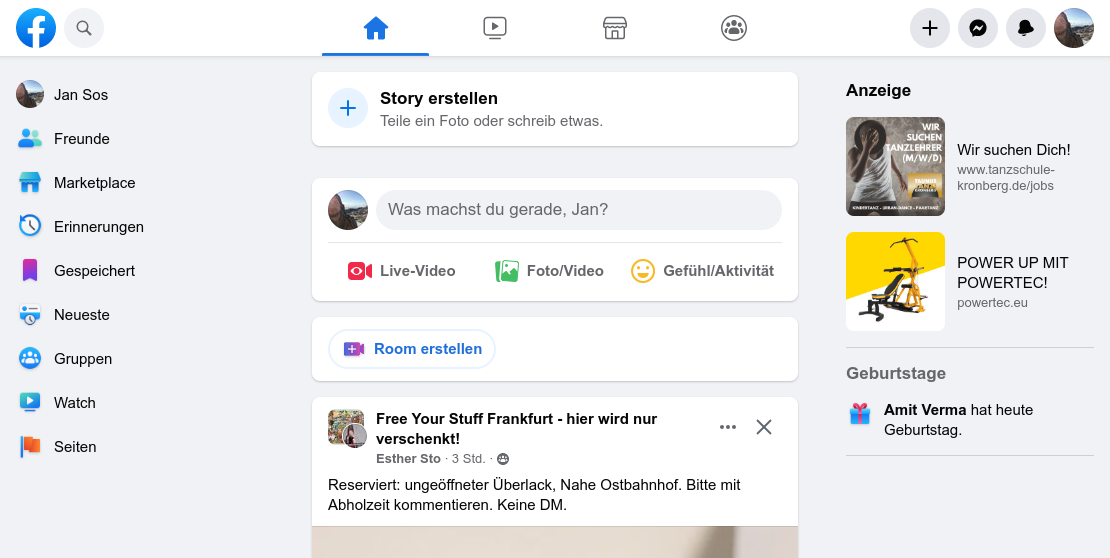
\includegraphics[width=\textwidth]{figures/jan/pic_facebook.png}
    \caption[Startseite von \acrshort{fb}]{Startseite von Startseite von \acrshort{fb}}
    \label{fig:facebook}
\end{figure}

Die Nutzung von \acrshort{fb} ist sehr vielfältig und hängt von den Bedürfnissen des einzelnen Nutzers ab. Neben reinen Darstellungs- und Austauschmöglichkeiten bietet \acrshort{fb} eine breite Palette von Anwendungen an, wie z.B. integrierte Video-, Game- und Datingportale sowie ein eigenes Bezahlsystem. Auf diese speziellen Anwendungen wird im weiteren Verlauf nicht weiter eingegangen.

\paragraph{Selbstdarstellung}

Für die Selbstdarstellung von Organisationen oder Personen bietet \acrshort{fb} ein eigenes Profil an, auf dem Bilder, persönliche Informationen und Vorlieben wie Musik öffentlich dargestellt werden können. Die Sichtbarkeit dieser Inhalte kann individuell angepasst werden. Neben den statischen Informationen enthält das Profil auch eine Pinnwand, auf der ältere und aktuelle Beiträge listenmäßig aufgeführt werden.

\paragraph{Formen des Austausches}

Beiträge ermöglichen den interaktiven Austausch und das Teilen von Momenten. Jeder Nutzer kann sie verfassen und auf seiner eigenen sowie auf fremden Pinnwänden veröffentlichen. Ereignisse wie das Hochladen von neuen Bildern generieren automatisch einen Beitrag, um Bekannte, Follower und andere Personen über Neuigkeiten im Profil zu informieren. Beiträge lassen sich neben einfachem Text auch mit Bildern oder Videos sowie mit Tags (Orte, GPS, Veranstaltungen, Personen, etc.) spezifizieren. Andere Nutzer können Beiträge kommentieren oder bewerten.

\acrshort{fb}-Gruppen ermöglichen den Austausch mit mehreren Personen zu gemeinsamen Themen. Ähnlich wie Profile haben Gruppen einen statischen Teil, in dem Administratoren eine Kurzbeschreibung der Gruppe veröffentlichen. Eine Pinnwand ermöglicht den Mitgliedern die Kommunikation untereinander. Durch das Erstellen von Events können Gruppenmitglieder gemeinsame Treffen oder Aktivitäten planen.\\
Gruppen werden sehr häufig und für verschiedene Themen genutzt. Insbesondere im städtischen Raum dienen sie zum Beispiel dem Verschenken von ungenutzten Dingen, dem Knüpfen neuer Kontakte in einer neuen Stadt oder dem Treffen von Menschen in der Nähe mit ähnlichen Hobbies. Auch der Austausch über diverse Themen in unterschiedlichen Bereichen auf regionaler, nationaler und internationaler Ebene ist weit verbreitet.

Der Austausch materieller Gegenstände findet hauptsächlich auf einem digitalen Marktplatz statt. Die geschalteten Anzeigen enthalten eine Überschrift, eine freie Beschreibung, Bilder, Angaben zum Zustand, zur Preisvorstellung, zum Ort und zum Herausgeber der Anzeige. Der Verfasser muss bei der Erstellung der Anzeige eine vordefinierte Kategorie auswählen, um die Auffindbarkeit zu erleichtern. Neben der direkten Kontaktaufnahme besteht für Interessenten die Möglichkeit, die Anzeige zu merken, mit einem Kontakt zu teilen oder einen Alarm zu erstellen, sobald ähnliche Produkte angeboten werden.

Auf \acrshort{fb} können Kontakte gepflegt werden, indem man sich gegenseitig in eine Freundesliste aufnimmt. Über diese Liste können Inhalte selektiv verteilt werden, so dass sie nur für \textit{Freunde} sichtbar sind. Zusätzlich werden \textit{Freunde} über das Dashboard gezielt informiert, wenn ein \textit{Freund} einen neuen Beitrag erstellt hat.

Für den direkten und privaten Austausch bietet \acrshort{fb} einen Chat an, in dem sowohl 1:1- als auch Gruppenchats möglich sind. Die Kommunikation erfolgt in Echtzeit und die Nachrichten können wie Beiträge Bilder, Links und andere Inhalte enthalten. In 1:1-Gesprächen besteht auch die Möglichkeit, Sprach- und Videoanrufe zu tätigen.

\paragraph{Neuigkeiten}

Um bei der Vielzahl der Beiträge und Reaktionen von Freunden oder Gruppen den Überblick zu behalten, bietet \acrshort{fb} ein Dashboard an, auf dem Neuigkeiten in Form einer endlosen und unsortierten Liste angezeigt werden. Das Dashboard enthält auch kommerzielle Werbung und Beiträge von Gruppen, die der Nutzer noch nicht abonniert hat, aber von Interesse sein könnten.

Neben dem Dashboard gibt es auch eine Notifications-Seite, die einen gezielteren Fokus auf das Wesentliche ermöglicht. Hier werden kurze Benachrichtigungen wie Geburtstage von \textit{Freunden}, bevorstehende Events, neue Beiträge aus abonnierten Gruppen sowie Reaktionen auf eigene oder kommentierte Beiträge angezeigt.

\paragraph{Recherche}

\acrshort{fb} bietet eine Suchfunktion, die es Nutzern ermöglicht, nach Personen, Gruppen und anderen Inhalten zu suchen. Die Suchergebnisse können durch verschiedene Filter wie Art des Inhalts, Verfasser, Gruppen, Zeitraum und mehr genauer spezifiziert werden.

Zusätzlich können Nutzer Beiträge und öffentliche Profile als \textit{Bookmarks} sichern. Die \textit{Bookmarks} können dann auf einer dafür vorgesehenen Seite je nach Typ aufgelistet und verwaltet werden.

\subsubsection{Nebenan.de}

Nebenan.de ist eine Plattform, die im Jahr 2015 gestartet wurde und wie \acrshort{fb} darauf abzielt, Menschen zu vernetzen (Abb. \ref{fig:nebenan}). Der Unterschied zu \acrshort{fb} besteht darin, dass sich Nebenan.de ausschließlich auf die unmittelbare Nachbarschaft des Nutzers konzentriert.

\begin{figure}[!htb]
    \centering
    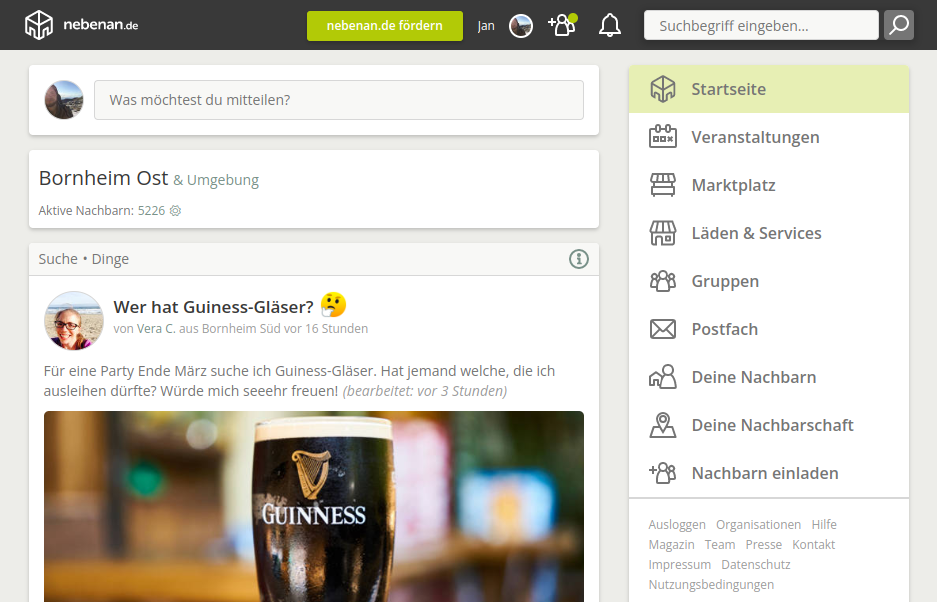
\includegraphics[width=\textwidth]{figures/jan/pic_nebenan.png}
    \caption[Startseite von nebenan.de]{Startseite von nebenan.de}
    \label{fig:nebenan}
\end{figure}

Die Zielgruppe umfasst alle Interessengruppen, die in der Nachbarschaft des Benutzers vertreten sind, wie z.B. Anwohner, Vereine, Firmen und Organisationen. Die Nachbarschaftsgrenze wird vom System anhand der eigenen Adresse des Nutzers definiert und kann nicht individuell angepasst werden.

\paragraph{Selbstdarstellung}

Für die Darstellung existieren auf Nebenan.de zwei Arten von Profilen. Die erste Profilart gilt für Einzelnutzer. Hierbei können sich Anwohner über ein Kurzprofil mit Foto, einem Freitext sowie ihren Interessen und Angeboten vorstellen. Zur Auswahl der Interessen und Angebote gibt es fest definierte Vorschläge, um zu beschreiben, was der Anwohner in die Nachbarschaft einbringen kann. Dazu zählen beispielsweise das \textit{Annehmen von Paketen}, das \textit{Blumengießen}, die \textit{Reparatur von Fahrrädern} oder das \textit{Gesellschaft leisten}. Das Profil zeigt auch die Aktivitäten des Anwohners an, wie beispielsweise beigetretene nebenan-Gruppen und die Anzahl der erhaltenen virtuellen Dankeschöns. \\
Organisationen und Läden/Services, die vor Ort angesiedelt sind und zum alltäglichen Leben in der Nachbarschaft beitragen, nutzen die zweite Profilart. Diese Profile enthalten im Vergleich zu den Anwohnerprofilen deutlich mehr Informationen und müssen beim Anlegen einer Kategorie zugeordnet werden, wie z.B. \textit{Restaurant}, \textit{Reisen}, \textit{Sport}, \textit{Political Party} oder \textit{Nachbarschaftsinitiative}. Neben grundlegenden Informationen wie Name, Adresse, Kontaktdaten und Öffnungszeiten können auch zukünftige Veranstaltungen, Gesuche, Bekanntmachungen, das Verkaufsangebot und weitere Informationen hinterlegt werden. Anwohner können auf den öffentlichen Profilen ihre eigenen Erfahrungen mit der Organisation oder dem Laden teilen und Empfehlungen aussprechen.

\paragraph{Formen des Austausches}

Nebenan.de nutzt den Beitrag als zentrales Mittel für den Austausch zwischen Anwohnern. Jeder Beitrag kann von allen Anwohnern kommentiert und positiv bewertet werden. Beiträge werden bei der Erstellung einer Kategorie zugeordnet, um zu kennzeichnen, ob es sich um ein \textit{allgemeines Thema}, ein \textit{Gesuch}, ein \textit{Angebot}, eine \textit{Empfehlung} oder eine \textit{Veranstaltung} handelt. Jede Kategorie wird in mehrere aufeinander aufbauende Unterkategorien unterteilt, um die Beiträge besser einordnen zu können. \\
Abhängig von der Art des Beitrags werden diese entweder auf dem öffentlichen Dashboard, dem Event-Feed oder dem Marktplatz angezeigt. Ein Beitrag besteht aus einem Titel, einem Freitext und optionalen Bildern. Bei Veranstaltungen können weitere Felder wie Datum und Ort hinzugefügt werden \\
Die Beiträge auf dem Marktplatz werden neben der Hauptkategorie \textit{Angebot} noch weiter in die Unterkategorien wie \textit{Hilfe}, \textit{Schenken}, \textit{Verleihen} oder \textit{Tauschen} unterteilt. Verkaufsangebote können zudem weiter spezifiziert werden, indem sie einer Angebotskategorie wie \textit{Essen}, \textit{Baby \& Kinder} oder \textit{Haustiere} zugeordnet werden. Alle Angebote sind in einer Liste verfügbar und können nach Kategorie gefiltert oder mithilfe der globalen Suchfunktion durchsucht werden.

Um den Austausch unter Menschen mit gemeinsamen Interessen zu erleichtern, bietet nebenan.de die Möglichkeit, Gruppen zu erstellen. Dabei kann der Zweck der Gruppe durch einen aussagekräftigen Namen und eine Beschreibung genauer erläutert werden. In diesen Gruppen können Mitglieder verschiedene Arten von Beiträgen wie Mitteilungen, Suchanfragen, Angeboten oder Veranstaltungshinweisen veröffentlichen. Diese Beiträge erscheinen auf der Gruppenpinnwand und können von allen Gruppenmitgliedern kommentiert werden.

Neben der Gruppenfunktion gibt es auch eine Chatfunktion für den direkten Austausch mit einzelnen Nutzern. Mit dieser Funktion können Nutzer neben reinem Text und Emojis auch Fotos und Empfehlungen verschicken.

\paragraph{Neuigkeiten}

Für die Anzeige von neuen Beiträge steht ein Nachbarschafts-Dashboard zur Verfügung. Hier werden alle Arten von Beiträgen nach dem Datum der letzten Änderung sortiert angezeigt. Der Austausch mit der Nachbarschaft findet hauptsächlich über das Dashboard statt, wo neue Beiträge entdeckt und beantwortet werden können. \\
Zusätzlich werden alle Beiträge, an denen man aktiv teilgenommen hat und bei denen neue Ereignisse aufgetreten sind, nochmals separat in einem Benachrichtungs-Feed aufgelistet, um einen besseren Überblick zu gewährleisten. Darüber hinaus werden im Benachrichtigungs-Feed alle zukünftigen Veranstaltungen in der Nachbarschaft angezeigt.

\paragraph{Recherche}

Die nebenan-Suche bietet eine Möglichkeit zur Suche von Beiträgen jeglicher Art. Interessante Beiträge oder solche, die wichtige Informationen für den Benutzer enthalten, können als Lesezeichen gespeichert werden. Diese Lesezeichen können je nach Art des Beitrages unter \textit{Feed} oder \textit{Marktplatz} eingesehen und bei Bedarf gelöscht werden.

\subsubsection{Spontacts}

Spontacts konzentriert sich im Gegensatz zu \acrshort{fb} und Nebenan.de ausschließlich auf die Organisation von Freizeitaktivitäten für Menschen in der gleichen Region (vgl. Abb. \ref{fig:spontacts}). Die Plattform richtet sich insbesondere an Personen, die Gleichgesinnte für bestimmte Aktivitäten suchen und dabei neue Kontakte knüpfen möchten.

\begin{figure}[!htb]
    \centering
    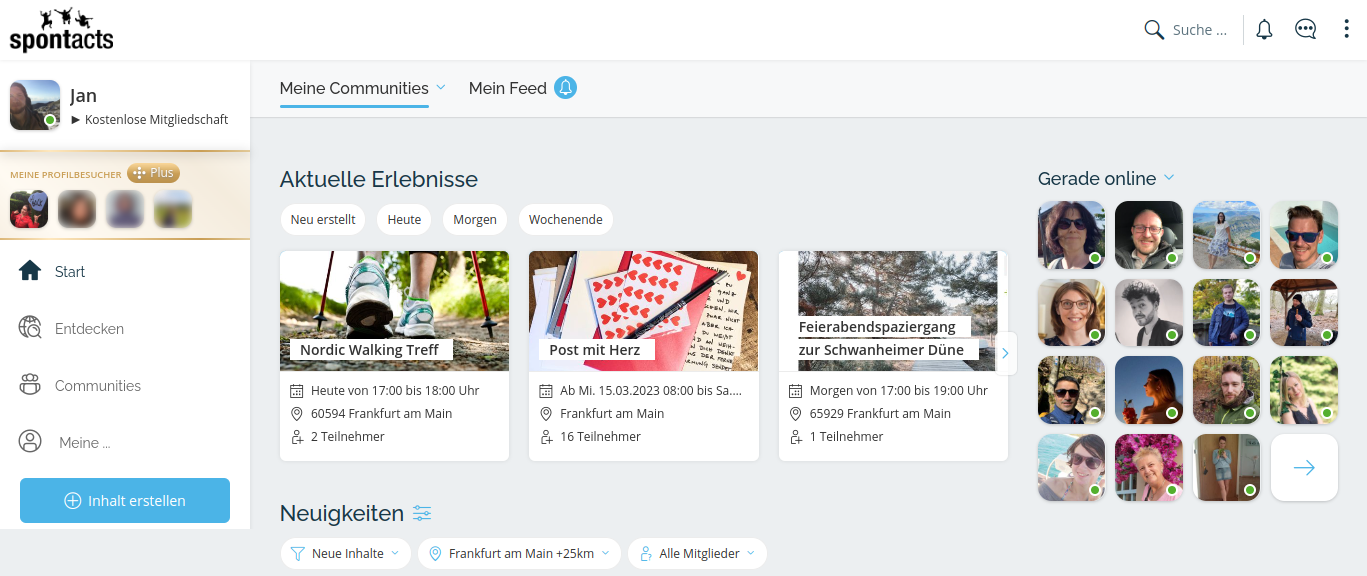
\includegraphics[width=\textwidth]{figures/jan/pic_spontacts.png}
    \caption[Startseite von Spontacts]{Startseite von Spontacts}
    \label{fig:spontacts}
\end{figure}

\paragraph{Selbstdarstellung}

Das Nutzerprofil auf Spontacts ähnelt dem anderer vergleichbarer Anwendungen und beinhaltet grundlegende Informationen wie den Namen, ein Profilbild, das Alter und den Wohnort. Es können jedoch auch weitere Angaben wie präferierte Kontakte für \textit{Freizeit}, \textit{Sport}, \textit{Reisen}, \textit{Tanzen} und \textit{Dating} oder zusätzliche Profilabschnitte (Hobbies, Interessen/Vorlieben usw.) hinzugefügt werden. Ein weiterer Abschnitt zeigt vergangene und zukünftige Aktivitäten des Nutzers sowie dessen Gruppenmitgliedschaften an.

\paragraph{Formen des Austausches}

Zur Interaktion mit anderen Benutzern können Beiträge in Spontacts erstellt werden. Diese Beiträge können je nach Art als einfacher Beitrag, als Aktivität oder als Frage/Diskussion verfasst werden und werden dann in Communities, Gruppen oder gegebenenfalls in Foren angezeigt. Wie gewohnt können sie kommentiert, gelikt und geteilt werden.

Die Communities sind eine Art Oberkategorie, die einen bestimmten Themenbereich (\textit{Ausgehen \&\ Party}, \textit{Essen \&\ Trinken}, \textit{Natur \&\ Umwelt} usw.) beschreiben und jedem Beitrag zugeordnet werden. Beim Erstellen einer Gruppe muss daher immer eine passende Community ausgewählt werden. Im Gegensatz zu den anderen vorgestellten Diensten sind Gruppen bei Spontacts das zentrale Feature der Anwendung. Sie ähneln in ihrem Funktionsumfang den Gruppen auf \acrshort{fb}.

Über die Beiträge hinaus können die Nutzer auch über den Chat eine private Unterhaltung führen. In diesem Chat können ausschließlich Textnachrichten ausgetauscht werden.

\paragraph{Recherche}

Um Beiträge, Veranstaltungen, Gruppen, Mitglieder und mehr zu entdecken, bietet Spontacts eine Suchfunktion mit spezifischen Filteroptionen je nach dem gesuchten Typ. Der Nutzer kann neben den allgemeinen Einstellungen wie Suchbegriff, Umkreis und Erstelldatum auch objektspezifische Kriterien wie Veranstaltungsdatum, Alter und ähnliches hinzufügen, um die Suche zu verfeinern.

Mitglieder können in die Kontakt- oder Merkliste aufgenommen werden, wenn sie für den Nutzer von Interesse sind. Die Merkliste ist eine private Liste, in die jedes Mitglied aufgenommen werden. Die Kontaktliste hingegen ist öffentlich und erfordert eine Bestätigung der Anfrage durch die betreffende Person. \\
Zusätzlich besteht die Möglichkeit, anderen Mitgliedern zu folgen, um ihre Aktivitäten besser verfolgen zu können. Wer wem folgt, kann in jedem Benutzerprofil eingesehen werden.

\paragraph{Neuigkeiten}

Um innerhalb der Plattform auf dem Laufenden zu bleiben, gibt es wie bei anderen Portalen ein Dashboard für Gruppen/Communities sowie einen Benachrichtigungs-Feed. Im Dashboard werden in der Rubrik \textit{Neuigkeiten} alle anstehenden Veranstaltungen und aktuellen Inhalte der Communities dargestellt. Unter der Rubrik \textit{Mein Feed} können hingegen alle Veränderungen in beigetretenen Gruppen eingesehen werden, wie beispielsweise neue Mitglieder und Veranstaltungen.\\
Der Benachrichtigungs-Feed enthält Informationen über neue Kontaktanfragen, Beiträge aus den Gruppen und Neuigkeiten über die Plattform.

\subsection{Strategische Ausrichtung}

Die drei Hauptwettbewerber weisen viele Gemeinsamkeiten auf, unterscheiden sich jedoch in ihrer strategischen Ausrichtung voneinander.

\acrshort{fb} ist eine sehr aktive Plattform, die sich darauf konzentriert, Menschen mit beliebigen Interessen, Themen und Bedürfnissen zu vernetzen, ohne dass der Nutzer dabei auf einen bestimmten geografischen Raum beschränkt ist. In letzter Zeit konnte keine intensive Weiterentwicklung der Plattform beobachtet werden, da sich das Unternehmen hauptsächlich der Entwicklung von zukünftigen Produkten im 3D-Umfeld widmet. Es ist daher lang- und mittelfristig keine Veränderung zu erwarten.

Nebenan.de ist der größte Konkurrent von \acrshort{dht}. Die Plattform ermöglicht es den Nutzern, sich in ihrer Nachbarschaft auszutauschen und zu vernetzen, wobei der Fokus auf der Stärkung der Gemeinschaft liegt. Eine große Herausforderung für Nebenan.de besteht darin, eine lebendige Community aufzubauen, die alle gesellschaftlichen Schichten und Altersklassen ansprechen.

Im Gegensatz dazu konzentriert sich Spontacts stark darauf, Menschen im privaten Bereich für gemeinsame Aktivitäten zu vernetzen. Die Plattform hat eine aktive Community, in der Nutzer Inhalte erstellen und an allen Veranstaltungen teilnehmen können, ohne harte lokale Einschränkungen wie bei nebenan.de. Darüber hinaus werden die Inhalte der Seite von lokal ansässigen Moderatoren betreut, die zusätzliche Veranstaltungen organisieren und durchführen. Strategisch setzt Spontacts zunehmend auf kostenpflichtige Accounts, die den Nutzern zusätzliche Funktionen wie verbesserte Filterfunktionen bieten sollen.

\subsection{Zusammenfassung}

Nach der Analyse der Konkurrenz wurde deutlich, dass die untersuchten Dienste ähnliche Funktionen wie Profile, Gruppen und Chats bereitstellen. Die Unterschiede zwischen den Features liegen eher in Nuancen, die von den jeweiligen Betreibern individuell gestaltet werden. \\
Die Plattformen unterscheiden sich jedoch in Bezug auf ihre Motivationen, Zielgruppen und geografischen Nutzerbereiche stark voneinander. Während einige Plattformen sich auf bestimmte Nachbarschaften beschränken, decken andere globale Communities ab. \\
Im Gegensatz dazu konzentriert sich \acrshort{dht} gezielt auf die Region/Gemeinde. Dadurch füllt \acrshort{dht} die Lücke zwischen \acrshort{fb} als weltweitem Akteur und nebenan.de mit Fokus auf die Nachbarschaft.

%Darüber hinaus hebt sich \acrshort{dht} von anderen Diensten durch die Einbindung von Vereinen und öffentlichen Einrichtungen ab, die die Plattform zur Kommunikation mit den Anwohnern nutzen können.

Ein weiterer Aspekt, der sich bei einem direkten Vergleich deutlich zeigt, ist die unterschiedliche Benutzerfreundlichkeit und Nutzerführung auf den verschiedenen Plattformen. Teils sind Inhalte schwer auffindbar und die zugrunde liegenden Konzepte sind nicht immer selbsterklärend. Um sicherzustellen, dass \acrshort{dht} für alle Altersgruppen verständlich ist, ist es unerlässlich, eine Plattform zu entwickeln, die einfach strukturiert und intuitiv zu bedienen ist.

Die Analyse zeigt anhand von nebenan.de und Spontacts, dass der Aufbau und die Etablierung eines sozialen Netzwerks viele Herausforderungen mit sich bringen. Als Vorreiter hat sich \acrshort{fb} in der Gesellschaft bereits stark etabliert und bietet mit einer breiten Palette von Features vielseitige Nutzungsmöglichkeiten für unterschiedliche Bedürfnisse. \\
Insbesondere für neue Plattformen stellt der Aufbau einer Community eine große Herausforderung dar. Als Newcomer müssen sie ohne bereits vorhandene Community und Content meist mit ähnlichen Funktionen wie Facebook die Nutzer überzeugen, dass ihre Plattform einen spürbaren Mehrwert im Vergleich zu Facebook bietet.
Gerade bei Plattformen, bei denen die Nutzer ausschließlich die Inhalte erstellen, gestaltet sich der Aufbau einer Community als besonders zäh, da neue Nutzer aufgrund mangelnder Inhalte schnell wieder abwandern können.\\
Daher ist es essentiell, dass kontinuierlich neue Inhalte zur Verfügung stehen, um sich zu etablieren. Spontacts setzt hierfür gezielt Moderatoren ein, um seinen Nutzern regelmäßig Angebote zu präsentieren. Alternativ kann die Bindung an ein Portal auch durch Angebote von Dritten erfolgen, wie zum Beispiel durch regelmäßige Informationen von Vereinen, Stadtverwaltungen oder Zeitungen, wie es bei \acrshort{dht} geplant ist. Zusätzliche Funktionen, wie ein Buchungsportal, können den Nutzern auch bei bestimmten Aktivitäten unterstützen.

\section{Anforderungsanalyse}
\label{sec:requirementanalysis}
% \section{Requirementsanalysis}

Die Anforderungsanalyse ist ein entscheidender Schritt im Software-Entwicklungsprozess, der dazu beiträgt, die Bedürfnisse der Nutzer zu identifizieren und zu verstehen. Um jedoch die Bedürfnisse der Nutzer vollständig zu verstehen, ist es notwendig, eine detaillierte Analyse der Geschäftsanforderungen durchzuführen. Das Value Proposition Canvas bietet dabei eine effektive Methode zur Identifizierung der Kundenbedürfnisse und zur Entwicklung von wertvollen Produkten und Services. Dieses Kapitel befasst sich mit der Anforderungsanalyse mit dem Hilfsmittel des Value Proposition Canvas.

\subsection{Value Proposition Canvas}

Die Anforderungsanalyse nach dem Value Proposition Canvas ist ein Prozess, bei dem die Bedürfnisse und Anforderungen der Kunden identifiziert und dokumentiert werden, um sicherzustellen, dass das Unternehmen Produkte oder Dienstleistungen anbietet, die einen hohen Nutzen für die Kunden bieten.

\begin{figure}
    \centering
    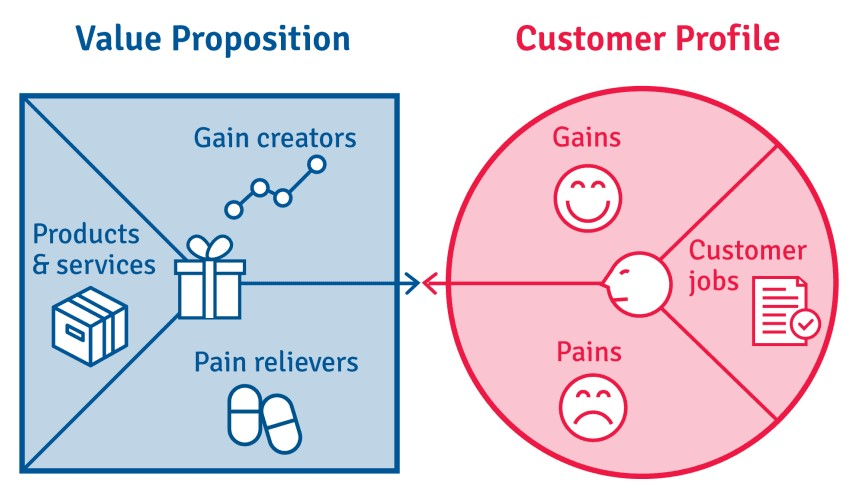
\includegraphics[width=0.6\textwidth]{figures/andre/valuepropositioncanvas.jpg}
    \caption{Value Proposition Canvas}
    \label{fig:valuepropositioncanvas}
\end{figure}

Der Value Proposition Canvas besteht aus zwei Hauptbereichen:

\begin{itemize}
    \item[1.]	Der Kundenprofilbereich: In diesem Bereich identifizieren Sie die Bedürfnisse und Anforderungen Ihrer Zielgruppe und erstellen ein detailliertes Profil der Kundenperspektive.
    \item[2.]	Der Value-Map-Bereich: In diesem Bereich legen Sie fest, wie Ihr Produkt oder Ihre Dienstleistung den Kundenbedarf erfüllt und welche Vorteile es im Vergleich zu anderen Lösungen bietet.
\end{itemize}

\subsection*{Vorgehensweise}

Um eine erfolgreiche Analyse nach dem Value Proposition Canvas durchzuführen, sollten folgende Schritte beachtet werden:

\begin{itemize}
    \item[1.] Kundenprofilbereich 
    \begin{itemize}
        \item Identifizierung der Bedürfnisse und Herausforderungen der Zielgruppe
        \item Definierung der Kundenperspektive und Erstellen eines Profils für die Zielgruppe
    \end{itemize}
    \item[2.] Value-Map-Bereich
    \begin{itemize}
            \item Definition der Produkte oder Dienstleistungen, die angeboten werden sollen
            \item Festlegung der Vorteile, die das Produkt gegenüber anderen Konkurrenten bieten könnte
            \item Sicherstellung, dass die Bedürfnisse der Zielgruppe erfüllt werden
    \end{itemize}
\end{itemize}

\subsection{Personas und Zielgruppe}
Zu Beginn des Projekts wurde bereits die initiale Zielgruppe definiert. Da eine Social Media Plattform grundsätzlich ein potentiell sehr breites Spektrum an Nutzern besitzt, wurde die Entscheidung der Zielgruppe anhand dem bestmöglichen erreichen vieler Menschen definiert: Junge Erwachsene und Vereine - unter Betrachtung eines eher ländlicheren Landkreises.

Junge Erwachsene sind in der Regel affin und offener für den Umgang mit Technik, bei Erfolg der Plattform könnten diese wiederum über persönliche Kontakte und Werbung weitere Nutzer auf die Plattform ziehen. Vereine besitzen in der Regel bereits ein Netzwerk und bieten gleichzeitig die Möglichkeit, Menschen mit ähnlichen Interessen miteinander zu verknüpfen.

\subsection{Profile}
Um die Zielgruppen abbilden zu können, wurden insgesamt 4 Profile definiert, diese wurden nach dem Value Proposition Canvas analysiert und daraus jeweils Features abgeleitet. Diese sollen im Folgenden beschrieben werden:
\subsection*{Musikverein}
Beim Musikverein wird angenommen, es handelt sich um einen existierenden Verein mit einer funktionierenden Vorstandschaft und einer lebhaften Mitgliedschaft.
Dieser hat nach dem Value Proposition Design die folgenden Eigenschaften:


\subsection*{Alleinstehender Erwachsener Mann, frisch zugezogen}
Bei dieser Person handelt es sich um einen jungen alleinstehenden Mann, der erst wenige Wochen im Ort wohnt um eine neue Arbeit anzutreten. Dieser kennt nur das nötigste, ist zwar technikaffin, aber handwerklich nicht sonderlich begabt.

\subsection*{Alleinstehende Frau mittleren Alters}
Diese Frau ist alleinstehend, geschieden und Vollzeit berufstätig. Sie hat 2 jugendliche Kinder welche bei ihr wohnen und ist auf der Suche nach einem neuen Lebenspartner. Sie ist Mitglied in einem Gartenbauverein in der Gemeinde.

\subsection*{Junges Pärchen}
Mit diesem Profil soll ein junges Pärchen abgebildet werden. Diese sind beide Mitte 20 und leben in ihrer ersten gemeinsamen Wohnung. Beide sind voll berufstätig und daher zeitlich sehr eingeschränkt. Beide studieren und würden ihr wissen gerne mit anderen teilen.

\subsection{Abgeleitete Features}
Zusammen mit den Zielen aus der Aufgabenbeschreibung sowie den Erkenntnissen aus der Kundenanalyse des vorange-gangenen Kapitels wurden folgende Features abgeleitet.

\subsubsection{Persönliche und Vereinsprofile}
\label{sec:abgeleitetefeatures}
Im Vordergrund einer Social Media Plattform steht die Darstellung der eigenen Person. Daher war die Grundlage für die Plattform die Implementierung von Profilen.
Die Anforderungen für das Profil waren, sich kurz und knapp selbst beschreiben zu können. Die Einfachheit der Bedienung und damit für potentielle Profiländerungen sollte gegeben sein. Mit den Nutzerprofilen sollte nur das Interesse an der Person oder dem Verein geweckt werden, um im nächsten Schritt einen direkten Kontakt über die Chatfunktion zu ermöglichen.
Ein Schlüsselelement der Plattform ist das sogenannte Tag-System, ähnlich dem bekannten Hash-Tag von Netzwerken wie bspw. Twitter. Über die Tags kann ein Nutzer seine Hobbys und Interessenfelder kurz und knapp angeben.
Zusätzlich zum Tag sollte auch die Möglichkeit gegeben sein, sich selbst über einen Freitext beschreiben zu können.
Die Option ein Profilbild hochladen zu können ist ebenfalls eines der Basis-Anforderungen die das System haben muss.

\begin{figure}[ht!]
    \centering
    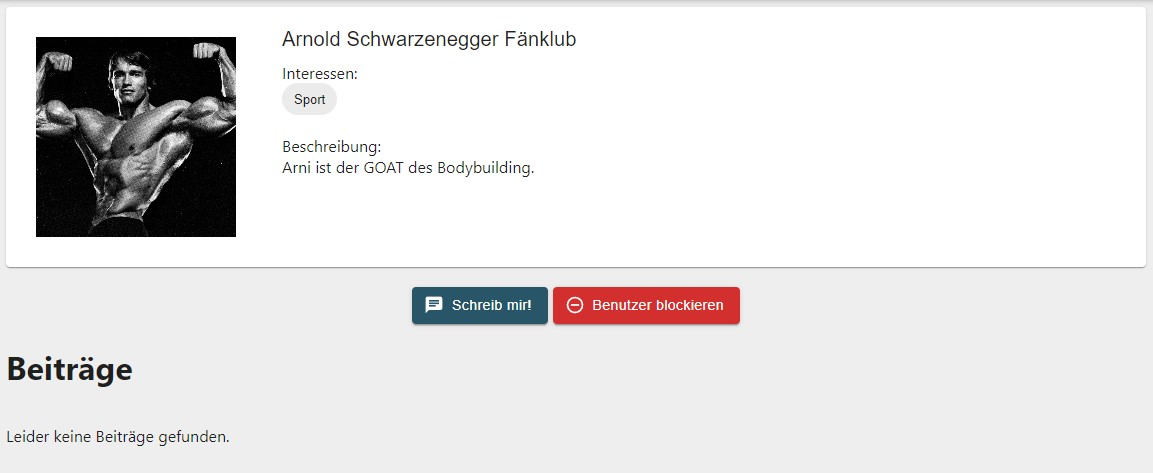
\includegraphics[width=0.6\textwidth]{figures/andre/beispielprofil.jpg}
    \caption{Beispielprofil}
    \label{fig:beispielprofil}
\end{figure}

In der obigen Abbildung ist ein Beispielhaftes Profil zu sehen. Es kann kurz und knapp auf das Thema der Organisation, in diesem Fall ein Fanclub über Arnold Schwarzenegger, abgeleitet werden. Des Weiteren sind auf dem Profil auch die erstellten Beiträge zu finden, ebenso wie eine Möglichkeit direkten Kontakt aufnehmen zu können. 

\subsubsection{Chats und Chaträume}
Ebenso obligatorisch wie die Profile ist auch die Chatfunktion, die zur Kontaktaufnahme unabdingbar ist. 
Auch hier stand wieder die Einfachheit im Fokus. Dies kann dadurch begründet werden, dass die Plattform nur zum Kennenlernen und Vernetzen der Menschen gedacht ist.
Ebenfalls soll die Möglichkeit bestehen, Gruppenchats zu erstellen. Dadurch kann man sowohl den Privatpersonen als auch Vereinen eine Möglichkeit geben sich in Gruppen zu organisieren. 

\begin{figure}[ht!]
    \centering
    \includegraphics[width=0.6\textwidth]{figures/andre/chatsundchaträume.jpg}
    \caption{Chats in Digital Dahoam}
    \label{fig:chatsundchaträume}
\end{figure}

\subsubsection{Beiträge, Veranstaltungen und Events}
Ebenfalls wichtig zur Kommunikation und Selbstdarstellung ist das Erstellen von Beiträgen. 

Aufgrund der Anforderungen wurden hierfür 4 Kategorien an Beiträgen herauskristallisiert:

\begin{itemize}
    \item	\textbf{Angebot} Man bietet etwas an, wie bspw. Hilfeleistung bei handwerklichen Tätigkeiten
    \item	\textbf{Anfrage} Hilfegesuch zu einem bestimmten Thema
    \item   \textbf{Information} Allgemeine Mitteilung
    \item 	\textbf{Veranstaltung} Teilen einer bevorstehenden Veranstaltung
\end{itemize}

Durch diese Kategorien können grundlegend die meisten Bedürfnisse zufriedengestellt werden. Es gibt sowohl die Möglichkeit, sich auszutauschen, als auch die Möglichkeit aktiv bzw. passiv nach Hilfe in der Nachbarschaft zu suchen bzw. diese anzubieten. Vereine können ihre Events mit der Öffentlichkeit teilen.

\subsubsection{Marktplatz und Entdecken}

Aufbauend auf den Beiträgen soll der Nutzer die Möglichkeit haben, gezielt nach eben jenen suchen zu können. Dies soll über das Explorationstool der Website ermöglicht werden.
Die Anforderungen hierfür waren, dass grundsätzlich nach allem und jedem gesucht bzw. gefiltert werden kann, anhand der zugewiesenen Tags. Dadurch kann dem Nutzer ermöglicht werden, auch wirklich nur die Beiträge zu sehen, die ihn auch Interessieren.
Des Weiteren sollten basierend auf demselben Prinzip (Tags) auch Personen gefunden werden können. Es wurde hierbei bewusst auf eine Klarnamensuche verzichtet, mit dem Ziel so möglichst viele neue Bekanntschaften zu ermöglichen. 

\begin{figure}[h!]
    \centering
    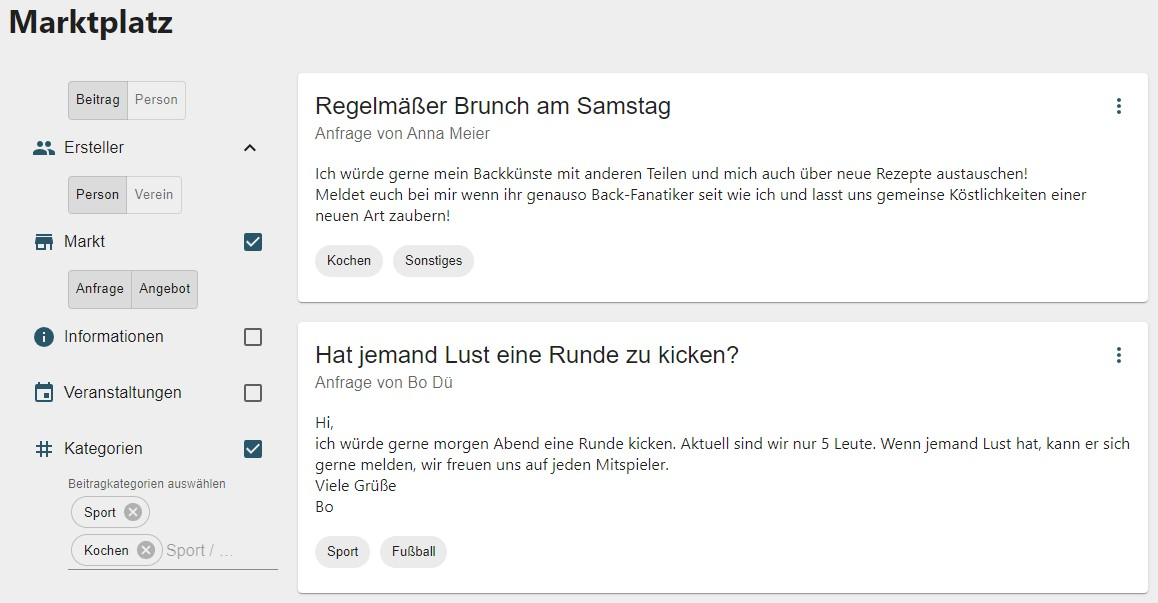
\includegraphics[width=0.6\textwidth]{figures/andre/marktplatzvondigitaldahoam.jpg}
    \caption{Marktplatz von Digital Dahoam}
    \label{fig:marktplatzvondigitaldahoam}
\end{figure}

\subsubsection{Persönlicher Merkzettel}
Als weiteres Feature sollte ein sog. Merkzettel implementiert werden. Dieser stellte sich als unabdingbar notwendig heraus für den Fall, dass ein Nutzer eine Veranstaltung sieht an der er interessiert ist und für später merken möch-te.
Aus dieser Anforderung wurde das allgemeine Feature des Merkzettels implementiert, sodass grundsätzlich die Möglichkeit gegeben ist, sich alle Beiträge merken zu können. Ähnlich wie beim Marktplatz kann auch hier nach den verschiedenen Beitragstypen gefiltert werden.

\begin{figure}[ht!]
    \centering
    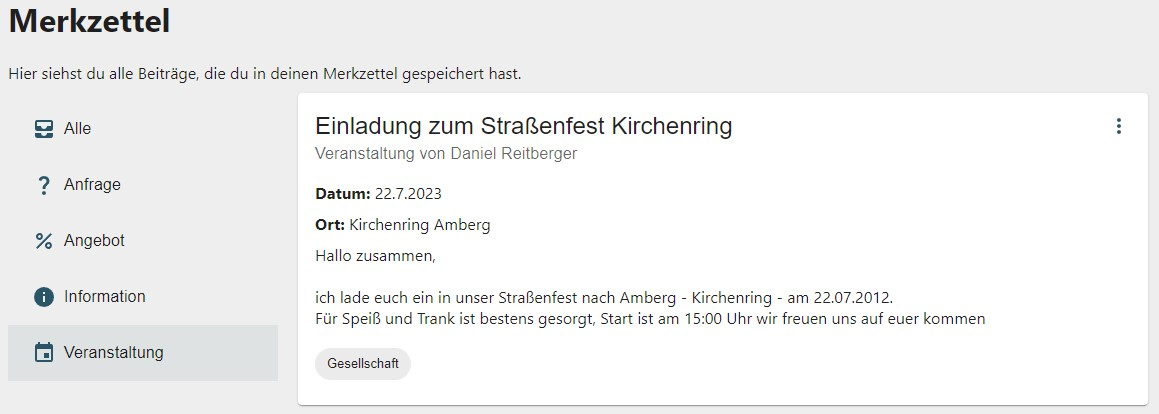
\includegraphics[width=0.6\textwidth]{figures/andre/merkzettel.jpg}
    \caption{Merkzettel}
    \label{fig:merkzettel}
\end{figure}

\section{Visuelle Grundstrukturen}
\label{sec:visualstructure}
% \section{Visuelle Grundstrukturen}

Ein wichtiger Faktor für den Erfolg des Scrum-Teams ist es, dass jeder im Team das gleiche Verständnis über das zu entwickelnde Produkt hat. Die Sicherstellung dessen ist von hoher Bedeutung, um vermeidbaren Zeitfressern, wie lange Diskussionen, Missverständnisse, Nacharbeit und eine \ggf daraus hervorgehende Demotivation im Team entgegenzuwirken.
Darüber hinaus entstehen durch eine Visualisierung des Produktes Ideen und Lösungsansätze für Abläufe und Features, die frühzeitig im Entwicklungsprozess angesprochen, diskutiert und eingearbeitet werden können, ohne einen bemerkbaren Mehraufwand zu generieren.
Wireframes eignen sich für diese Aufgabe sehr gut, da sich diese schnell erstellen und abändern lassen und zugleich jedem Teammitglied einen ersten Entwurf des Produktes aufzeigen. Ein weiterer Vorteil besteht darin, dass bereits frühzeitig dem Kunden auf einfache Weise die ersten Designkonzepte vorgestellt werden können und dieser sein Feedback in einer frühen Entwicklungsphase mit einfließen lassen kann.

Das Erstellen von Wireframes beinhaltet zugleich, sich frühzeitig mit dem Aufbau und der Konzeption der Website auseinanderzusetzen. Aus diesem Grunde wird im weiteren Verlauf auch auf die Themen Seitenstruktur und Layout eingegangen.

\subsection{Grundlagen Seitenstruktur}

Die Seitenstruktur einer Website beschreibt die Art und Weise, wie die Inhalte einer Anwendung präsentiert, organisiert und verlinkt sind.

Die darzustellenden Informationen müssen daher nach Inhalt aufgeteilt und thematisch auf einzelnen Seiten organisiert werden. Jede Seite der Website besitzt somit ein klares Ziel, worüber sie informieren soll. Die einzelnen Seiten unterscheiden sich daher \bzgl ihres Ziels und Inhaltes. Jedoch existieren auf jeder Website eine Reihe von sogenannten Kernseiten, die oft aufzufinden sind. Klassische Seitentypen sind \bspw Startseite, Kontaktseite, Landingpage, Content- sowie Detailseiten.

Die Startseite, auch als Homepage bekannt, beschreibt die Seite, die den Startpunkt \bzw Ursprung einer Website darstellt. Von ihr aus kann über Verlinkungen zu allen Unterseiten navigiert werden.
Die Landingpage hingegen ist die erste Seite, die ein User wahrnimmt, wenn er von einem externen Link auf die Website geführt wird und eine Session beginnt. Die Landingpage wird oft für das Marketing hergezogen, um den Besucher für den Dienst zu begeistern und weitere Schritte anzuregen.
Die Contentseite hingegen gibt einen Überblick über die angebotenen Inhalte und verweist auf die zugehörige Detailseite, auf der die Inhalte detailliert aufgeführt sind.

Wie aus der Beschreibung der Seitentypen hervorgeht, werden die einzelnen Seiten zu unterschiedlichen Zeitpunkten oder in einer bestimmten Reihenfolge aufgerufen. Dies lässt sich auch als eine Art Hierarchie verstehen, die die einzelnen Seiten zueinander haben. Ob es sich hierbei um eine flache oder tiefe Hierarchie handelt, ist von der Navigationsstruktur abhängig. Allgemein werden häufig, wegen der besseren Orientierung, flache Seitenhierarchien empfohlen.

\begin{figure}
    \centering
    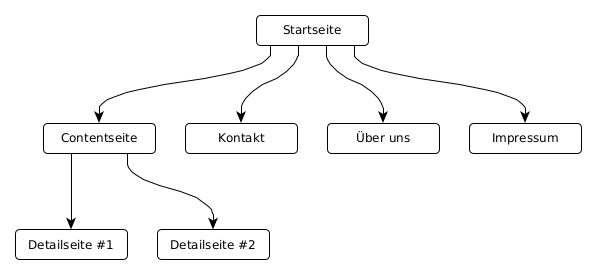
\includegraphics[width=\textwidth]{figures/jan/Wire_Hierarchie.png}
    \caption[Seitenstruktur einer Website]{Seitenstruktur einer Website}
    \label{fig:image}
\end{figure}

Die einzelnen Seiten einer Website unterscheiden sich jedoch \idR nicht vollständig voneinander. Sie folgen alle einem gleichbleibenden Aufbau. Dieses Grundgerüst einer Seite besteht oftmals aus einer Kopf- und Fußleiste und einem Inhaltsbereich. Die Kopf- und Fußleiste ist üblicherweise auf allen Seiten gleich ausgestaltet.

\begin{figure}
    \centering
    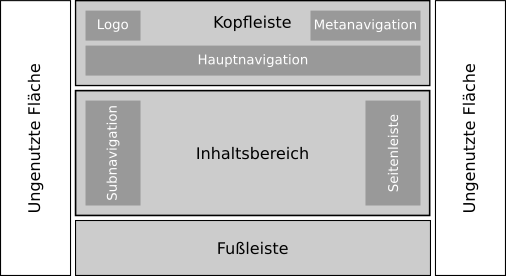
\includegraphics[]{figures/jan/Wire_Areas.png}
    \caption[Elemente einer Website]{Elemente einer Website}
    \label{fig:image}
\end{figure}

Der Kopfbereich einer Seite befindet sich im obersten Teil der Seite und umfasst das Logo, die Haupt- und Metanavigation. Der Kopfbereich wird häufig auch als Header bezeichnet.
Das Logo im Kopfbereich stellt ein wichtiges Erkennungs- und Differenzierungsmerkmal der Website dar und zielt auf das Erzeugen von Assoziationen mit der Website ab. Die Hauptnavigation gibt eine Übersicht über die verfügbaren Inhalte und stellt diese strukturiert dar. Die Hauptnavigation erweist sich für die Navigation als wichtigstes Element und wird häufig auffällig im oberen Bereich platziert. Eine weitere Navigationsleiste ist die Metanavigation, welche ergänzende Serviceinhalte wie \zB Accounteinstellungen der Seite verfügbar macht. Die Inhalte dieser Leiste haben keinen Bezug zu den Hauptthemen und werden daher gesondert aufgeführt.

Der Inhaltsbereich ist direkt unter dem Kopfbereich angeordnet und umfasst die zu vermittelnden Inhalte. Der Inhaltsbereich weist je nach Bedarf entweder nur die reinen Inhalte auf oder \ggf noch eine Subnavigation, die meist links angeordnet ist, sowie eine Seitenleiste (\engl Sidebar) für weiterführende Inhalte, die auf der rechten Seite untergebracht werden. Die zentralen Inhalte werden zwischen den Leisten, im sogenannten Inhaltsbereich, und meist nach Wichtigkeit absteigend sortiert aufgelistet.

Die untere Begrenzung der Internetseite bildet die Fußleiste (\engl Footer). Die Fußleiste beinhaltet meist Basisinformationen der Seite, ergänzende Inhalte oder auch \ggf weitere Navigationsmöglichkeiten.

Umschlossen werden die Seitenbereiche von einem umgebenden Block, der die ungenutzte Fläche der Website darstellt.

\subsection{Grundlagen Layout}
\subsection{Rastersystem}

Für die Überführung der ersten Skizzen in ein stimmiges Layout eignet sich die zur Hilfenahme eines Rastersystems. Ein Rastersystem stellt ein Netz mit Zeilen und Spalten dar, an welchen die Inhalte ausgerichtet und letztlich im Rastersystem platziert werden. Der Vorteil besteht darin, dass die Inhaltselemente und Einzelseiten in eine gleiche Struktur gebracht werden und die Seiten zunehmend abgestimmter und einheitlicher wirken. Das Raster wird lediglich für die Gestaltung herangezogen und sollte möglichst unauffällig oder dezent für den Endnutzer wirken,

Die Ausgangsbasis eines Rastersystems ist zu meist eine Leinwand mit definierten Abmessungen. Die Fläche wird in Spalten (\engl columns) unterteilt und \ggf wird zusätzlich noch zwischen den Spalten ein gleichbleibender Freiraum (\engl gutter) angelegt. Je höher die Spaltenanzahl gewählt wird, desto größer wird der gestalterische Spielraum, wobei der Nutzen des Rasters ab einer gewissen Anzahl zunehmend verschwindet.
In einem weiteren Schritt kann eine horizontale Unterteilung vorgenommen werden. Als Grundlage wird hier das sogenannte Baseline Grid verwendet, welches sich aus der Schriftgröße und dem Zeilenabstand zusammensetzt.
Die einzelnen Spalten und Zeilen können des Weiteren noch in Bereiche zusammengefasst werden, um ein modulares Rastersystem zu erstellen.
Die Website-Inhalte werden im Nachgang den Bereich zugeordnet und am Raster ausgerichtet.

\begin{figure}
    \centering
    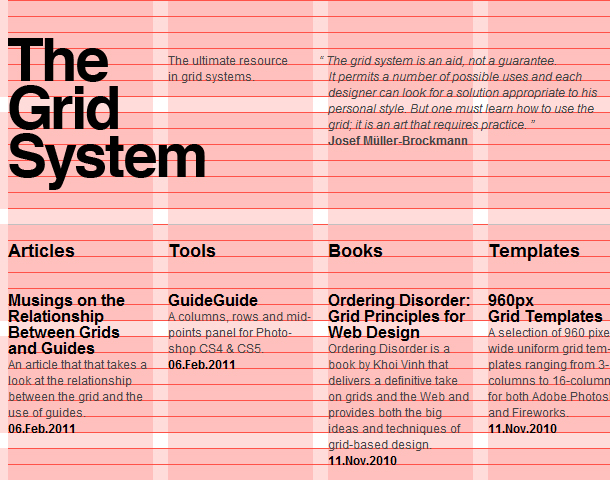
\includegraphics[width=0.6\textwidth]{figures/jan/Wire_Gridsystem.jpeg}
    \caption[Beispiel eines Rastersystems]{Beispiel eines Rastersystems}
    \label{fig:image}
\end{figure}

% ![Gridsystem](res/Wire_Gridsystem.jpeg)
% [//]: # (BILD Gridsystem: https://www.elmastudio.de/wp-content/uploads/2011/02/rastersysteme-webdesign-07.jpg)

\subsubsection*{Layouttypen}

Als es nur eine kleine Vielfalt an Endgeräten mit verschiedenen Auflösungen gab, wurde oft mit einem statischen Layout gearbeitet, welches für eine weit verbreitete Auflösung optimiert war. Heute lässt sich dieser Ansatz wegen der unüberschaubaren Menge an Geräten, die sich zudem stark in ihren Auflösungen unterscheiden, kaum noch heranziehen. Insbesondere schwer ist die Findung einer passenden Auflösung, die für einen Großteil der Geräte als ansprechend erscheint.
Heutzutage geht man hingegen nicht mehr von einer festen Breite bei der Layouterstellung aus, sondern erstellt Layouts, die sich je nach Auflösung individuell dem Gerät anpassen.

Während dieser Entwicklung sind verschiedene Layouttypen entstanden, die je nach Anwendungsfall zurate gezogen werden.

Das fixe Layout beschreibt einen Layouttyp, der mit festen Pixelwerten eine fixe Breite definiert. Bei einer passenden Auflösung werden alle Inhalte korrekt angezeigt. Je größer hingegen die Auflösung wird, desto größer wird der umgebende Block der Seite und viel ungenutzter Platz entsteht. Bei einer zu kleinen Auflösung tauchen horizontale Scrollbalken auf und die Inhalte erscheinen abgeschnitten \bzw werden nur noch unvollständig angezeigt.

\begin{figure}
    \centering
    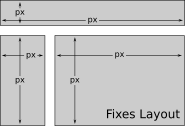
\includegraphics[scale=1.2]{figures/jan/Wire_Fixes-Layout.png}
    \hspace{0.05\textwidth}
    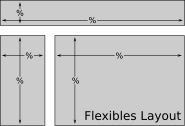
\includegraphics[scale=1.2]{figures/jan/Wire_Flexibles-Layout.png}
    \caption[Aufbau eines fixen und flexiblen Layouts]{Aufbau eines fixen und flexiblen Layouts}
    \label{fig:image}
\end{figure}

Das Gegenstück zum fixen Layout stellt das flexible Layout dar. Dieses passt sich allen Veränderungen unmittelbar an und behält dadurch zu jeder Zeit alle vorgegebenen Größenverhältnisse. Definiert wird es im Gegensatz zu den festen Pixelwerten mit relativen prozentualen Werten, wodurch es sich unterschiedlichen Varianten einer Website leicht anpassen kann. Der reine Layouttyp kommt jedoch eher selten zum Einsatz. Vielmehr lässt sich häufig eine Mischform aus fixem und flexiblem Layout vorfinden.

Eine weitere Layoutform ist das elastische Layout. Das elastische Layout verfolgt den Ansatz, dass sich die Inhalte einer Seite anpassen. Dieser Layouttyp ist besonders für Inhalte geeignet, die die vollständige Bildschirmbreite ausfüllen, was \bspw bei einer Produktpräsentation mit großformatigen Bildern und Videos der Fall ist. Die Inhalte müssen hierfür in der Lage sein sich automatisch flexibel anzupassen. Daher ist es für diese Form von Vorteil, wenn es eher wenige Inhalte zum Vorstellen gibt.

Auf Basis des flexiblen Layouts setzt das responsive Layout auf und erweitert die Möglichkeiten situationsgerecht ein passendes Layout für das Endgerät zur Verfügung zu stellen. Das responsive Layout besitzt als Erweiterung sogenannte Media-Queries, welche es ermöglichen beim Über- oder Unterschreiten fester Schwellwerte eine Veränderung der Ansicht zu starten und die Inhalte \bspw neu anzuordnen.

\subsection{Grundlagen Wireframes}

\subsubsection{Definition/ Inhalte}

Als Wireframe wird die schematische Darstellung von Inhalten und Elementen der Seitenoberfläche verstanden. Wireframes dienen insbesondere zur Konzeptionierung in der Planungsphase, um einerseits einen groben Entwurf für die Verteilung, Anordnung und Gestaltung von den Seitenelementen zu erhalten sowie zum anderen die Beziehungen zwischen den Seiten herzustellen.
Die Darstellung des Seitenlayouts ist zumeist eine skizzenhafte, in schwarz-weiß/ grau gehaltene Abbildung. Die einzelnen Bestandteile der Seite werden dabei durch einfache geometrische Formen verdeutlicht. Das Darstellen von Design, Farben, Schrift und Bilder ist kein Bestandteil der Methode. Ein fertiges Wireframe gibt dem Betrachter final Aufschluss über die Platzierung der Informationsinhalte, die Struktur und Navigation der Seite und die Interaktionselemente (Interface), mit welchen der Nutzer interagiert.
Die ausgearbeiteten Wireframes stellen weiter fort die Grundlage für die visuelle und funktionale Detaillierung des Produktes dar. Anschließende Schritte können \ua das Erstellen von Mockups oder Prototypen sein.

\subsubsection{Arten}

Wireframes werden allgemein in Low-Fidelity- und High-Fidelity-Wireframes unterschieden.
Low-Fidelity-Wireframes (LFW) stellen das klassische Verständnis von Wireframes dar, bei denen der Fokus allein auf dem funktionalen Design liegt. Die Seitenschemas werden mit einfachsten Formen und ohne konkrete Inhalte erstellt.
Die High-Fidelity-Wireframes (HFW) hingegen stellen die nächste Entwicklungsstufe für die Ausarbeitung des Designs dar. In ihr kommen zunehmend mehr und mehr Designkomponenten wie Farben, Typografie, Abstände, Icons, Text, Bilder und Grafiken zum Einsatz. In den Seiten werden zunehmend auch mehr reale Textlängen und Größenverhältnisse der Elemente und Inhalte mit einbezogen.

\begin{figure}
    \centering
    % [//]: # (BILD Beispiel LFW und HFW)
    % https://mentormate.com/blog/low-fidelity-wireframes-vs-high-fidelity-wireframes/
    % https://www.resolutesoftware.com/news/ux-wireframes/
    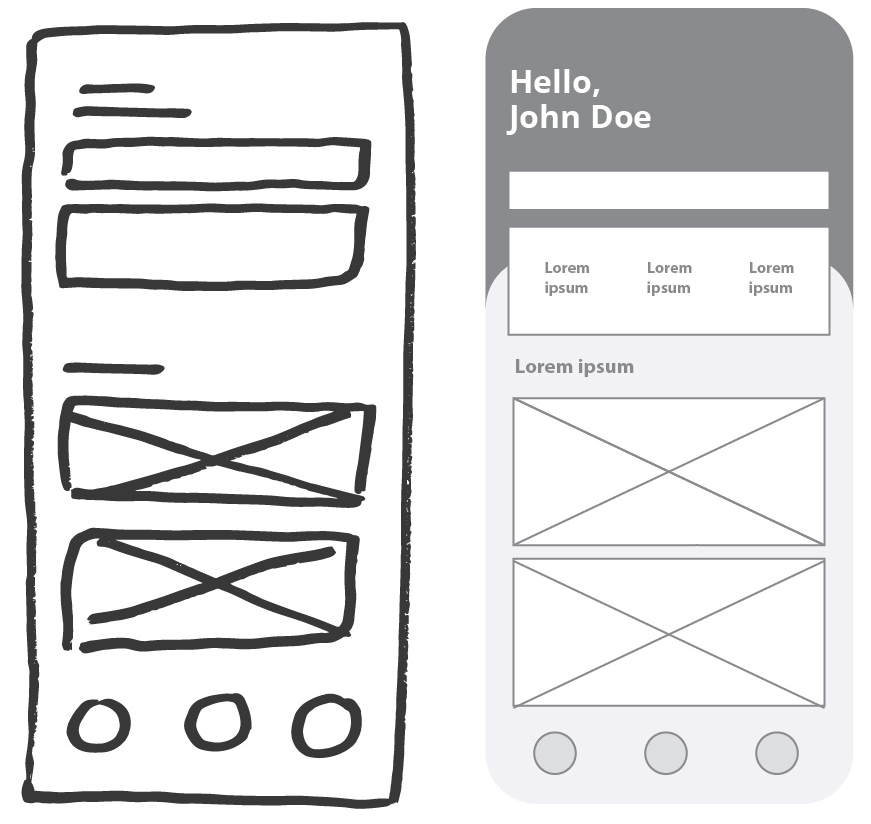
\includegraphics[scale=1]{figures/jan/Wire_Fixes-LFWvsHFW2.png}
    \caption[Beispielhafte Darstellung von LFW und HFW]{Beispielhafte Darstellung von LFW und HFW}
    \label{fig:image}
\end{figure}

\subsubsection{Abgrenzung}

Häufig werden im Zusammenhang mit Wireframes noch weitere visuelle Methoden in Verbindung gebracht. Weit verbreitet sind hier insbesondere Mockups und Prototypen. Diese Methoden verwenden jeweils Wireframes als Grundlage und zielen auf die zunehmende reale Veranschaulichung des zukünftigen Produktes.

Unter Mockups wird das Nachbilden eines Produktes oder auch ein maßstabsgerechtes Modell verstanden. Im Vordergrund der Methode steht das visuell-interaktive Design. Hierzu wird das Konzept der Wireframes übernommen und mit den Elementen der Benutzeroberflächen erweitert. Funktionale oder animierte Elemente sind nicht Bestandteil der Methode und werden nicht für einen Mockup aufgegriffen. Mockups werden im natürlichen Umfeld des Produktes dargestellt - zum Beispiel auf einem Gerätebildschirm. Das Ziel besteht darin das Produkt so echt wie möglich visuell nachzubilden, um dem Kunden ein reales Gefühl über die Erscheinung seines Produktes zu vermitteln.

% \begin{figure}
%     \centering
%     % [//]: # (Bild Mockup in Bildschirm)
%     \includegraphics[scale=0.25]{image.png}
%     \caption[]{image.png}
%     \label{fig:image}
% \end{figure}

Als Prototyp wird ein vereinfachtes Versuchsmodell des geplanten Produktes verstanden. Der Prototyp baut auf die Ergebnisse eines Mockups auf und erweitert dieses mit funktionalen Elementen, um die Interaktion eines Users mit dem Dienst simulieren zu können.
Ein klassisches Beispiel für einen Prototypen ist der Klick-Dummy. Ein Klick-Dummy ist ein teilweise interaktionsfähiges Demo einer Bedienoberfläche, welches alle relevanten Merkmale eines Produktes widerspiegelt und \ua zur Vorstellung oder für Testläufe genutzt werden kann.

\begin{figure}
    \centering
    % https://www.appschopper.com/blog/quick-guide-on-mobile-app-wireframe-vs-mockup-vs-prototype/
    % [//]: # (BILD Reihenfolge LFW - HFW - MockUp - Prototyp)
    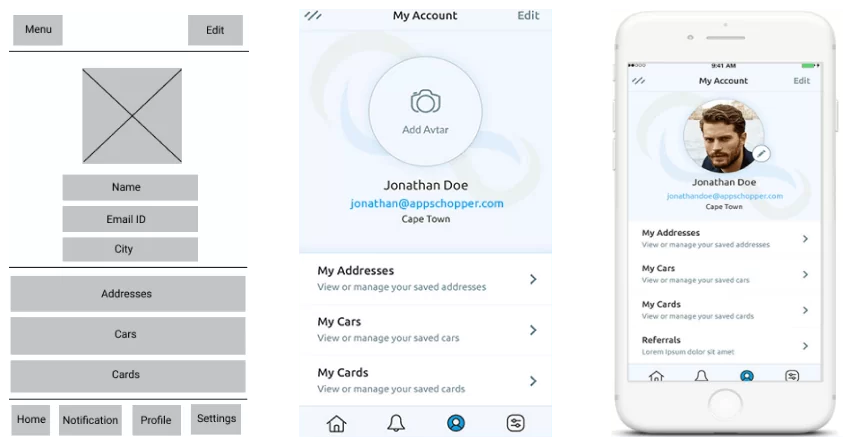
\includegraphics[scale=2]{figures/jan/Wire_Fixes-Wire-prototyp.png}
    \caption[Interationsschritte an einem Beispiel: Wireframe - Mockup - Prototyp]{Interationsschritte an einem Beispiel: Wireframe - Mockup - Prototyp}
    \label{fig:image}
\end{figure}

\subsection{Anwendung}
\subsubsection{Integration}

Die Wireframes wurden innerhalb des Projektverlaufes kontinuierlich für die Ausgestaltung und Kommunikation der User-Stories während des Backlog Refinement verwendet. Hierfür wurden in einer frühen Phase die jeweiligen User-Stories vom PO erläutert und ein erster Wireframe-Entwurf konzipiert. Erkenntnisse, die bereits während der Konzipierung entstanden, wurden an den PO übermittelt und nach Absprache noch während des Sprints direkt in die Wireframes aufgenommen.
Im Refinement dienten sie einerseits dem PO zur Vorstellung und Erklärung der User-Stories und andererseits zur Präzisierung und Detaillierung der Story im Team.
Die daraus neu gewonnenen Informationen wurden vom PO ins Backlog aufgenommen und erneut zum nächsten Refinement in die Wireframes eingearbeitet.

% \begin{figure}
%     \centering
%     % [//]: # (BILD Ablauf: Refinement 0 - 1 - 2 - 3, Feature A, B, C, Iteratives Vorgehen)
%     \includegraphics[scale=0.25]{image.png}
%     \caption[]{image.png}
%     \label{fig:image}
% \end{figure}

Neben der Definition und Veranschaulichung der jeweiligen Features wurden die Wireframes auch im Entwicklungsprozess herangezogen. In diesem wurden sie als gestalterischer Entwurf berücksichtigt und so weit wie es dem Entwickler möglich war, implementiert.

\subsubsection{Auswahl Tool}

Für die Erstellung von Wireframes stehen eine Vielzahl von verschiedenen Softwarelösungen zur Verfügung. Grundsätzlich lassen sich diese in desktop- und webbasierte Anwendungen unterscheiden. Für die Erstellung der Wireframes war es essenziell, dass diese leicht erstellt und angepasst werden können, \ggf auch paralleles Arbeiten möglich ist und dass das Teilen der aktuellen Entwürfe ohne zusätzlichen Aufwand geschieht. Anhand der Basisanforderungen konzentrierte sich die Auswahl zunehmend auf rein webbasierte Lösungen. Als Anbieter kristallisierte sich im weiteren Rechercheverlauf zunehmend Figma als ein passender Dienst heraus.

\begin{figure}
    \centering
    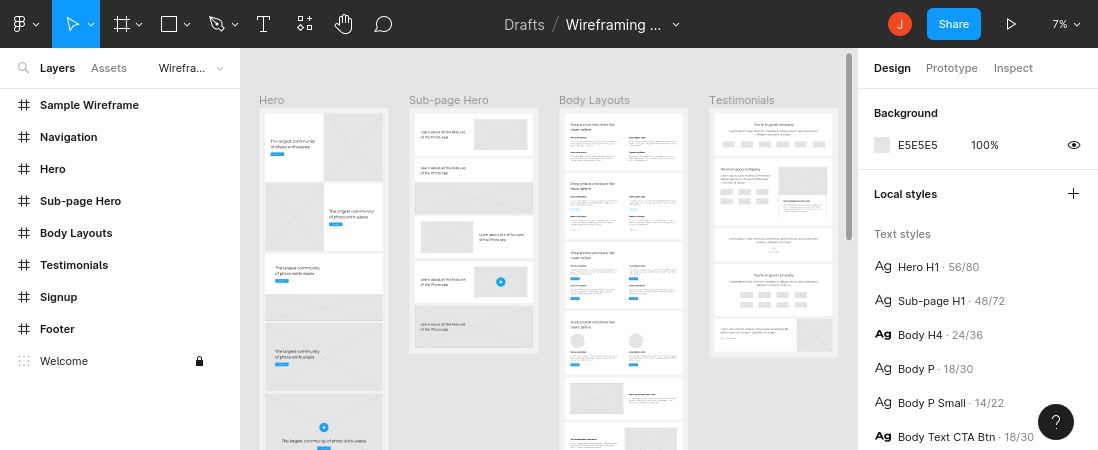
\includegraphics[width=\textwidth]{figures/jan/Wire_Figma.png}
    \caption[Figmas-Arbeitsumgebung]{Figmas-Arbeitsumgebung}
    \label{fig:figma}
\end{figure}

Figma ist eine Onlineanwendung, die sich auf die Erstellung von Wireframes, Mocks und Prototypen spezialisiert und sich in diesem Bereich etabliert hat. Gerade durch die Etablierung des Dienstes lässt sich schließen, dass es als Werkzeug ausgereift ist und die Erstellung einfacher Wireframes durchgängig unterstützt.
Für das Erstellen der Wireframes wurde sich auf die grundlegenden Funktionen von Figma beschränkt. Der verfolgte Ansatz während der Ausarbeitung mit Figma lag hierbei besonders auf der Beschränkung der wesentlichen Elemente, um die Kerninhalte der Features deutlich hervorzuheben. Eingesetzt wurden hierbei \ua zur Gestaltung die Elemente Rechtecke und Text sowie zur Orientierung und Ausrichtung der Inhaltselemente das Raster und die Gruppierfunktion.

\#\#\#\# Anforderungen an die GUI

Für die Ausarbeitung der Wireframes wurden vorab einige Anforderungen festgelegt, welche bei der Erstellung beachtet werden mussten. Die Anforderungen bezogen sich zum einen auf die Gestaltung der Oberfläche und zum anderen auf die technologiekonforme Gestaltung der Wireframes.

Eine wichtige Anforderung an die Plattform war es, die UI generationsübergreifend zu konzipieren. Aus diesem Ansatz heraus ließen sich die folgenden Ansprüche an die UI ableiten:

- Einfache und intuitive Seitengestaltung, um die Inhalte, den Funktionsumfang und die Bedienung schnell selbstständig erfassen zu können,
- Reduzierung der Inhalte auf das Wesentliche, um Verwirrungen/ Ablenkungen zu vermeiden,
- Flache Hierarchien, um direkte Zugriffe auf die gewünschten Inhalte zu ermöglichen.

Von der technologischen Seite her war es erforderlich, dass die erstellten Konzeptentwürfe sich auch mit den ausgewählten Web-Technologien umsetzen lassen. Die Entwickler sollten in die Lage versetzt werden die Entwürfe entweder mittels Eigenentwicklungen oder durch das Heranziehen von Bibliotheken umzusetzen, ohne auf größere Herausforderungen zu stoßen. Das Ziel war es darüber hinaus einen hohen Grad an Wiederverwendbarkeit der Komponenten zu erreichen.

\#\#\#\# Pages

Als geeigneter Wireframetyp wurde ein Hybrid aus LFW und HFW gewählt. Die erstellten Wireframes umfassten alle layouttypischen Bereiche wie Kopf-, Inhalts- und Fußbereich, deren Inhalte in Feldern vereinfacht symbolisiert wurden. Die einzelnen Felder beinhalteten Texte, Dummy-Blöcke \bspw für Bilder und Interaktionselemente (Buttons, Dialoge \usw).
Die Wireframes wurden sehr schlicht in Graustufen gehalten und ohne die Berücksichtigung von Designelementen (Farbe, Typografie \usw) erstellt. Für die regelmäßige Erstellung und Anordnung der Komponenten hat sich nach einigen Entwürfen die Leinwandbreite von 1160 Pixel mit einem Raster von 27×37 Pixel als vorteilhaft ergeben.

Wireframes wurden für die Seiten/ Dialoge

\begin{itemize}
    \item Landingpage,
    \item Registrierung,
    \item Dashboard,
    \item Chat,
    \item Profil,
    \item Accounteinstellungen,
    \item Merkzettel und
    \item Marktplatz
\end{itemize}

erstellt.

Die Art und Detailtiefe der Ausgestaltung zeigen exemplarisch die folgenden Wireframes.

\begin{figure}
    %\centering
    % https://latex.org/forum/viewtopic.php?t=29653
    \begin{minipage}[t]{0.5\textwidth}
        % [//]: # (BILD Wireframes)
        \includegraphics[page=2, width=1\textwidth]{figures/jan/wire_example.pdf}
        \caption[Startseite (DHT)]{Startseite (DHT)}
        \label{fig:image}
    \end{minipage}
    \begin{minipage}[t]{0.5\textwidth}
        % [//]: # (BILD Wireframes)
        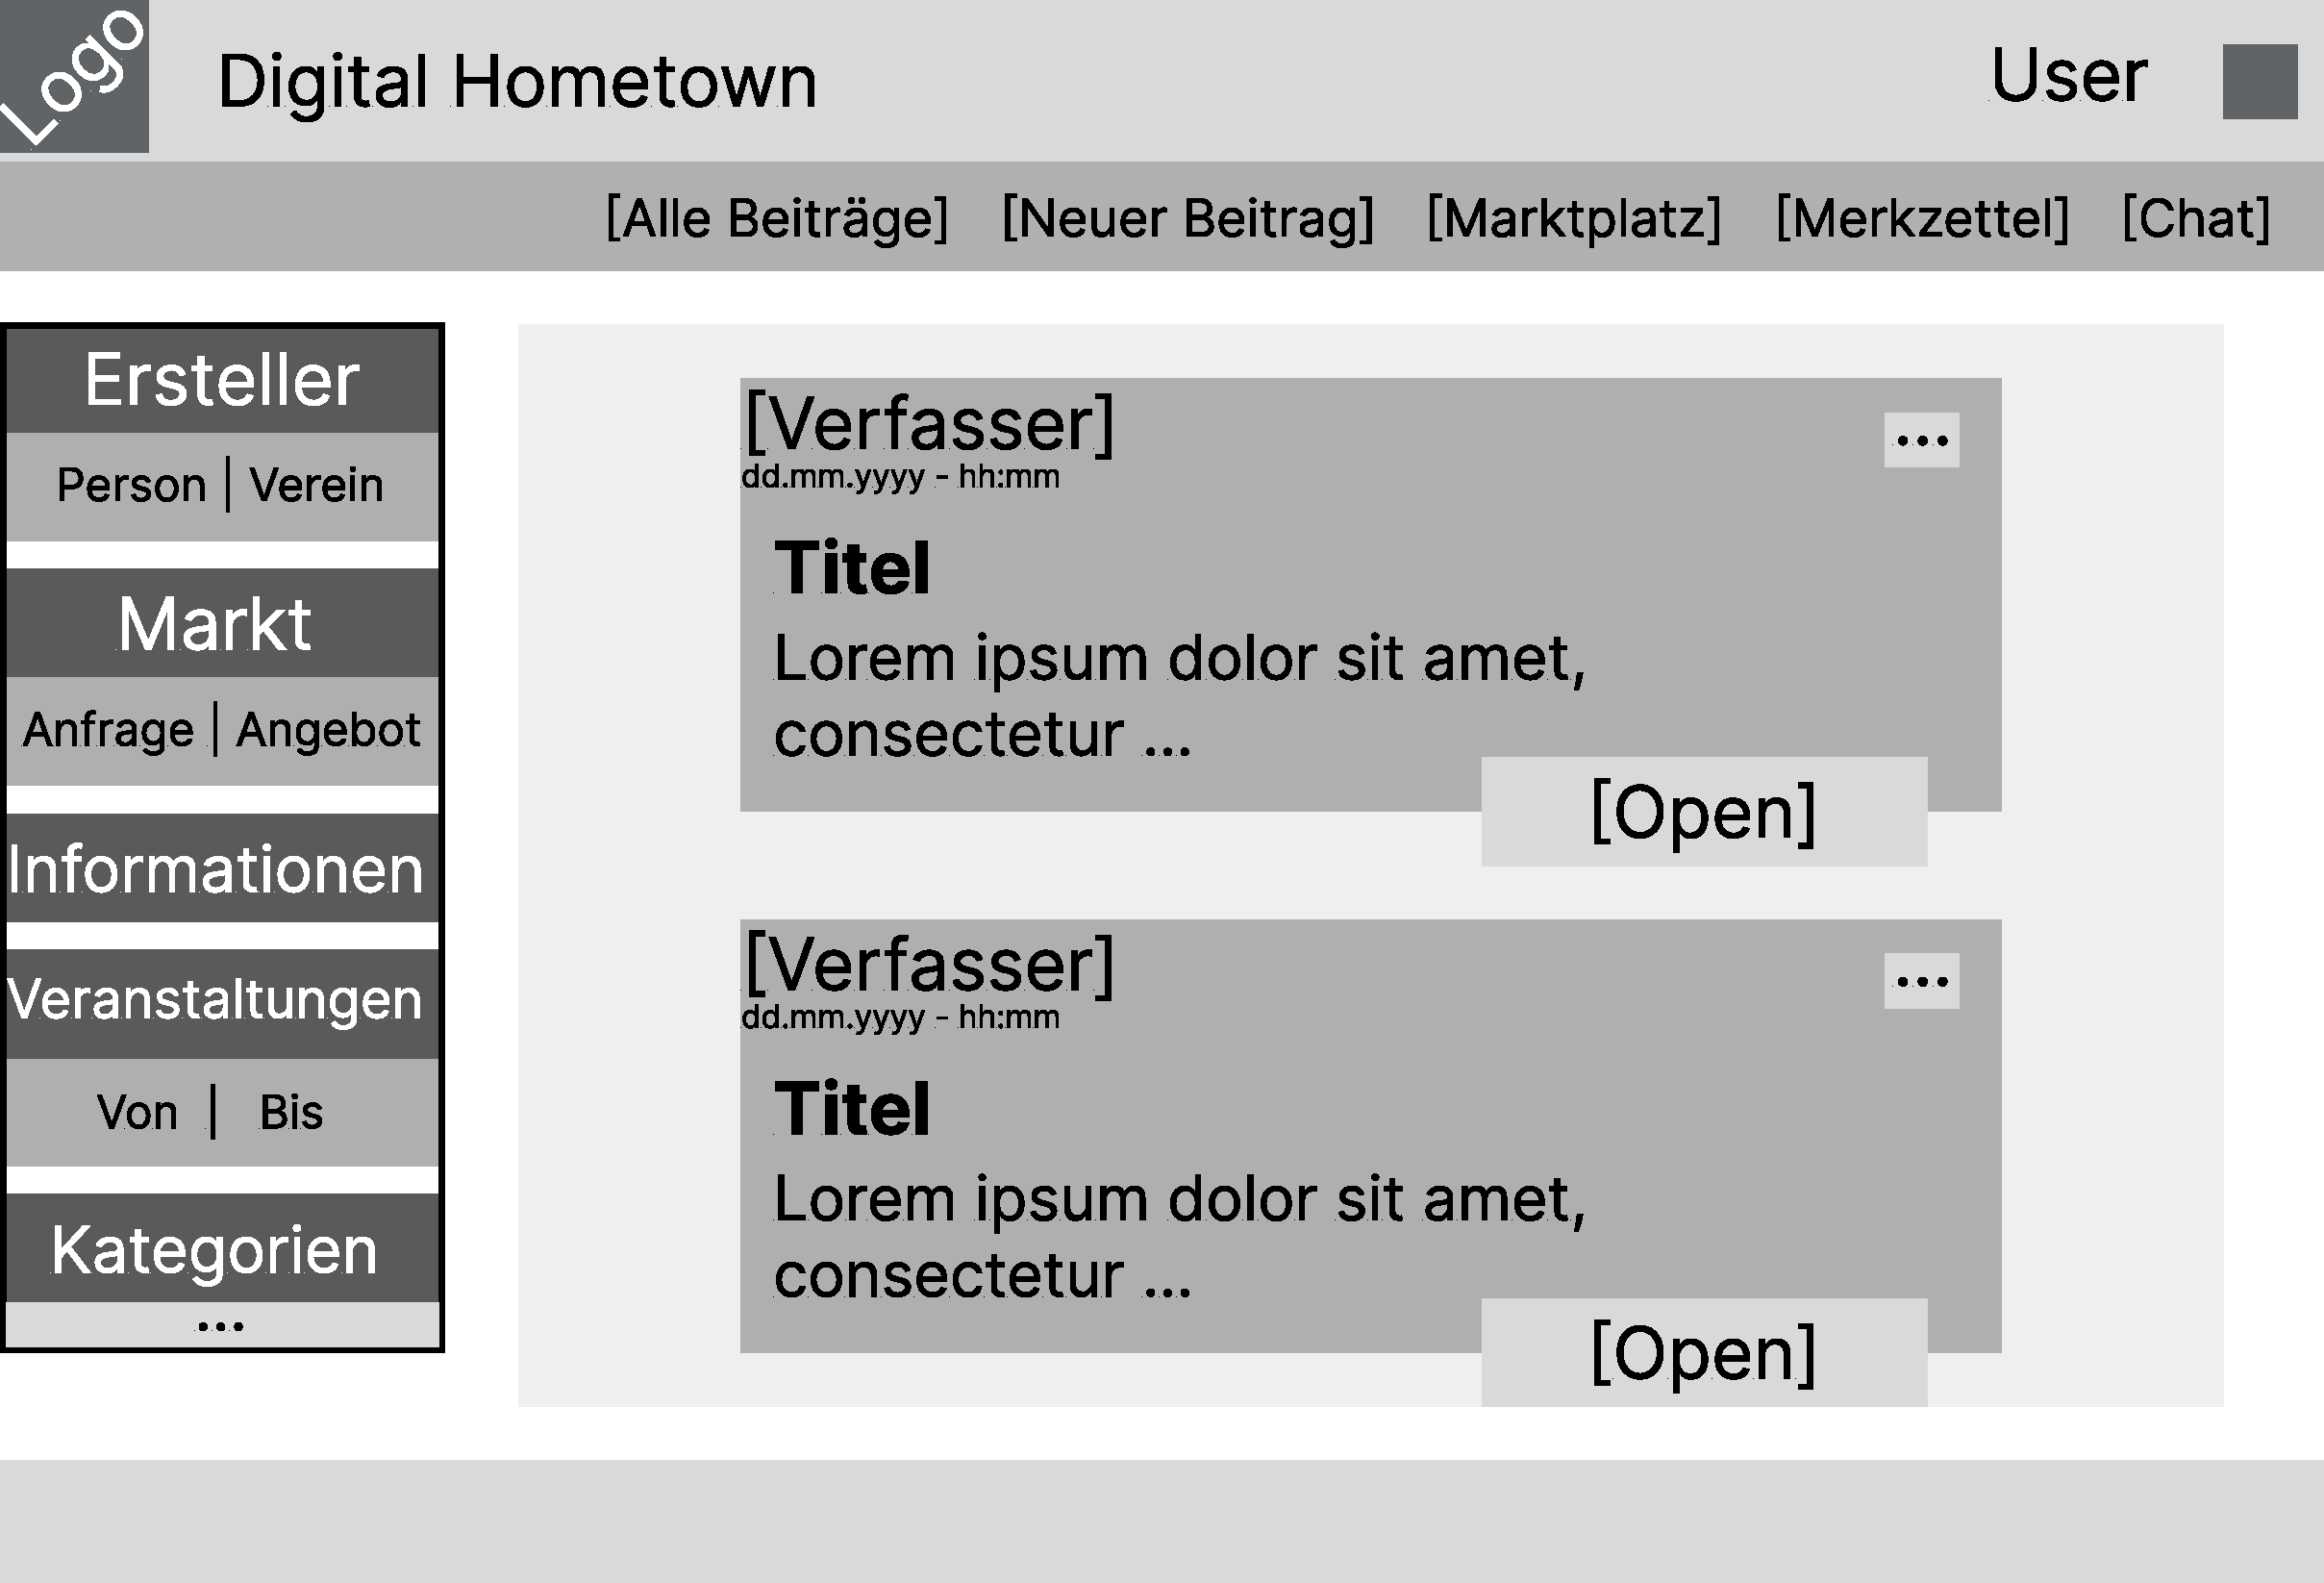
\includegraphics[page=1, width=1\textwidth]{figures/jan/wire_example.pdf}
        \caption[Marktplatz (DHT)]{Marktplatz (DHT)}
        \label{fig:image}
    \end{minipage}
\end{figure}


% \section{Usabilityanalyse}
% \label{sec:usabilityanalysis}

\section{Umfrage zur Digital-Hometown-Plattform}
\label{sec:umfrage}

Um die Plattform „Digital Hometown“ oder auch im Dokument als „Digital Dahoam“ tituliert optimal auf den Kunden auszurichten wurde im Folgenden eine Kurze Umfrage ins Leben gerufen um die Ansicht des Teams und des Kunden mit der realen Zielgruppe abzugleichen. Der Fragenkatalog wurde von mehr als 20 Personen unterschiedlichen Alters beantwortet und im Anschluss ausgewertet.

\subsection{Fragensammlung}

Neben den bereits entworfenen Personas wurde sich zu einem späteren Zeitpunkt des Projekts für die Durchführung einer Umfrage entschieden, mit dem Ziel die Bedürfnisse der Zielgruppe bestmöglich abzudecken. Hierfür wurde ein Fragebogen erstellt, bestehend aus 14 Aufgaben, welcher digital auszufüllen war. Neben einer kurzen Angabe des Alters wurden im Folgenden Präferenzen abgefragt bei der Benutzung und Bedienung einer digitalen Plattform. Ebenso wurde Inhalt somit priorisiert bzw. Features aus einer weiteren Sichtweise betrachtet. Auch Usability-Seitig wurden Anregungen entgegengenommen. Die Fragen selbst wurde als Team gemeinsam gesammelt.

\subsection{Auswertung}

Nach Abschluss der Umfrage nach einer halbwegs repräsentativen Anzahl an Teilnehmer wurden die Ergebnisse ausgewertet. Im Folgenden werden die Antworten je Fragestellung teilweise als Kreisdiagramm aber auch als Balkendiagramm dargestellt, je nach Themengebiet. Aus den gewonnenen Erkenntnissen wurden für die kommenden Sprints Themen und Features neu priorisiert und ebenso Fragestellung innerhalb der Umsetzung geklärt. Die Ergebnisse und die Wichtigkeit dieser Umfrage zeigt sich in der finalen Qualität der Homepage und des positiven Feedbacks seitens Kunde und Nutzer.

\begin{figure}[!htb]
    \centering
    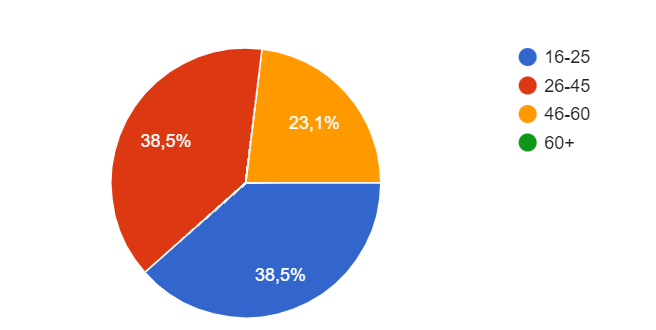
\includegraphics[width=1\textwidth]{figures/daniel/Bild-3.png}
    \caption[shortcaption]{Altersverteilung Umfrage}
    \label{fig:bild3}
\end{figure}

\begin{figure}[!htb]
    \centering
    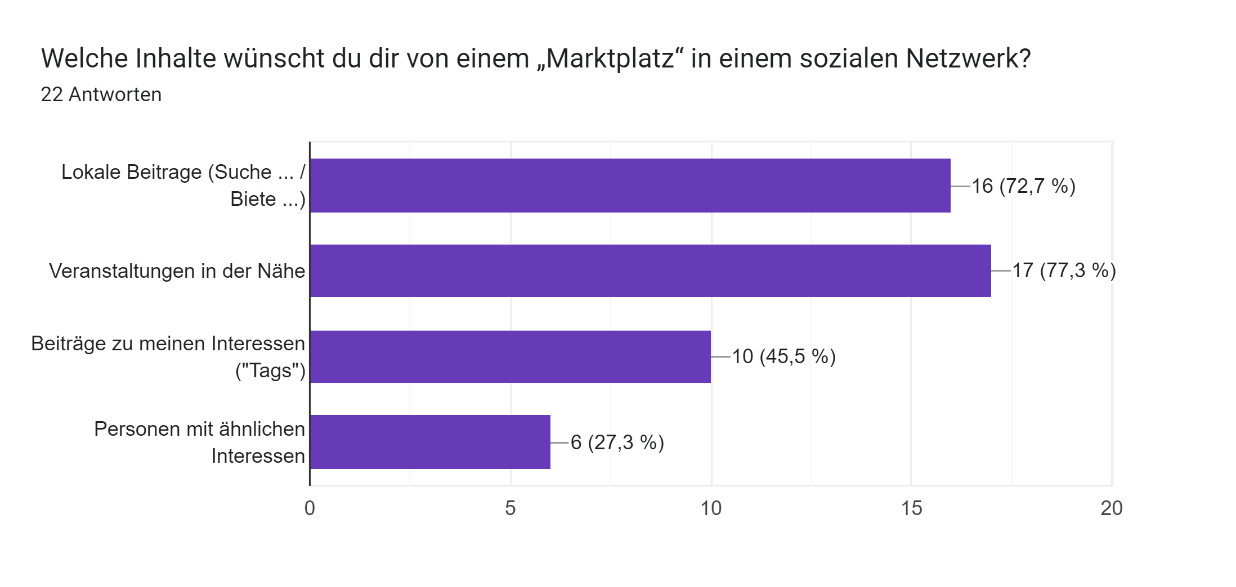
\includegraphics[width=1\textwidth]{figures/daniel/Bild-4.png}
    \caption[shortcaption]{Inhalte Marktplatz Umfrageergebnis}
    \label{fig:bild4}
\end{figure}

\begin{figure}[!htb]
    \centering
    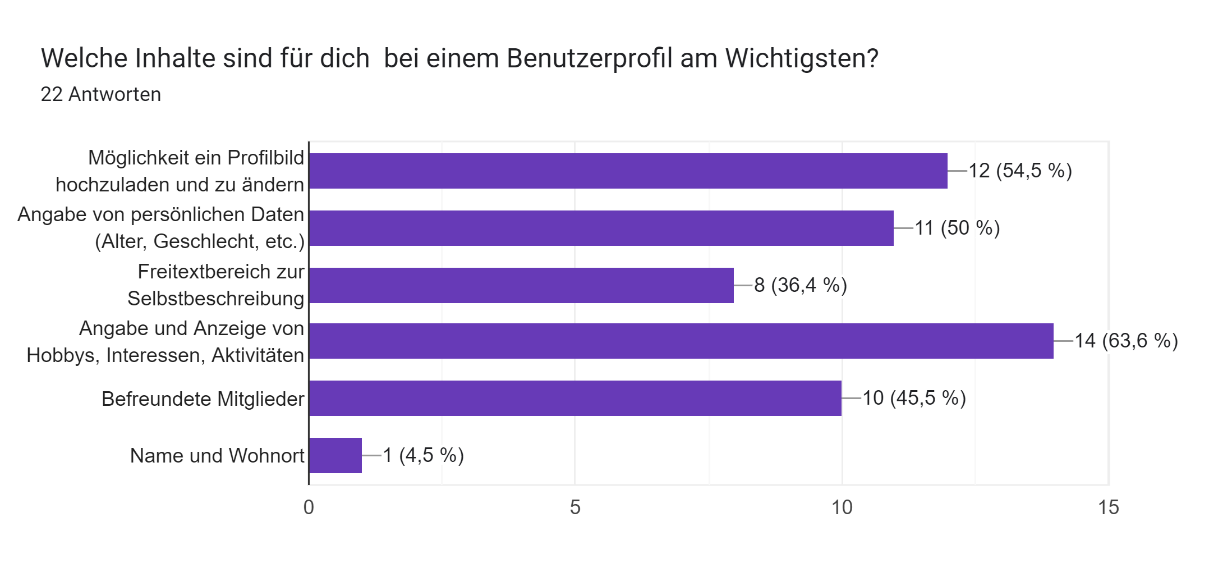
\includegraphics[width=1\textwidth]{figures/daniel/Bild-5.png}
    \caption[shortcaption]{Inhalte Benutzerprofil Umfrageergebnis}
    \label{fig:bild5}
\end{figure}

\begin{figure}[!htb]
    \centering
    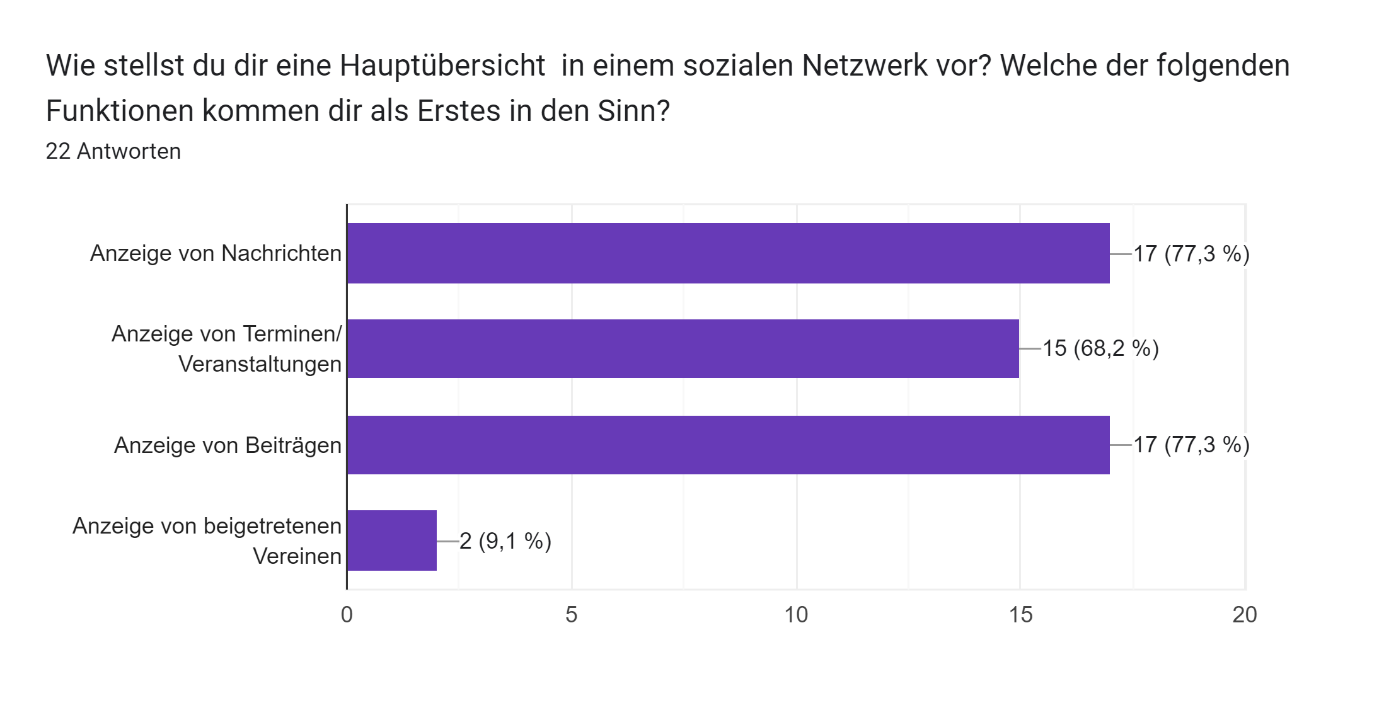
\includegraphics[width=1\textwidth]{figures/daniel/Bild-6.png}
    \caption[shortcaption]{Hauptübersicht Umfrageergebnis}
    \label{fig:bild6}
\end{figure}

\begin{figure}[!htb]
    \centering
    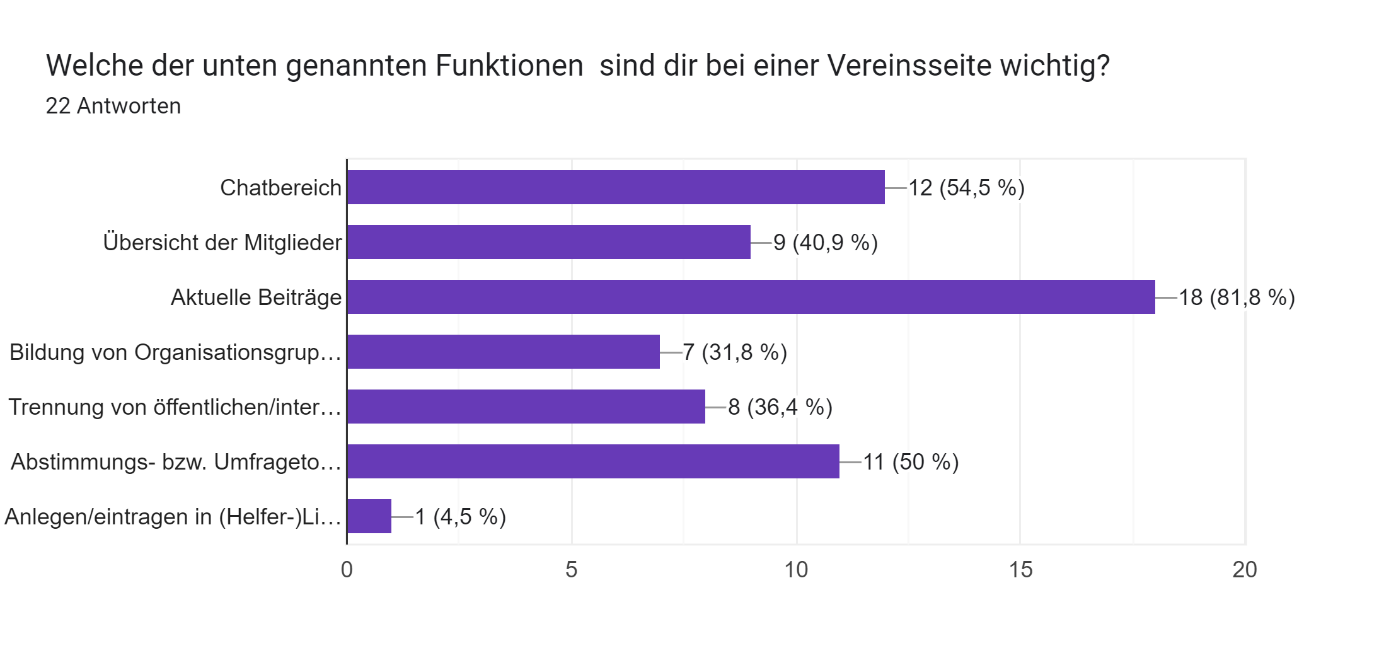
\includegraphics[width=1\textwidth]{figures/daniel/Bild-7.png}
    \caption[shortcaption]{Inhalte Vereinsseite Umfrageergebnis}
    \label{fig:bild7}
\end{figure}

\begin{figure}[!htb]
    \centering
    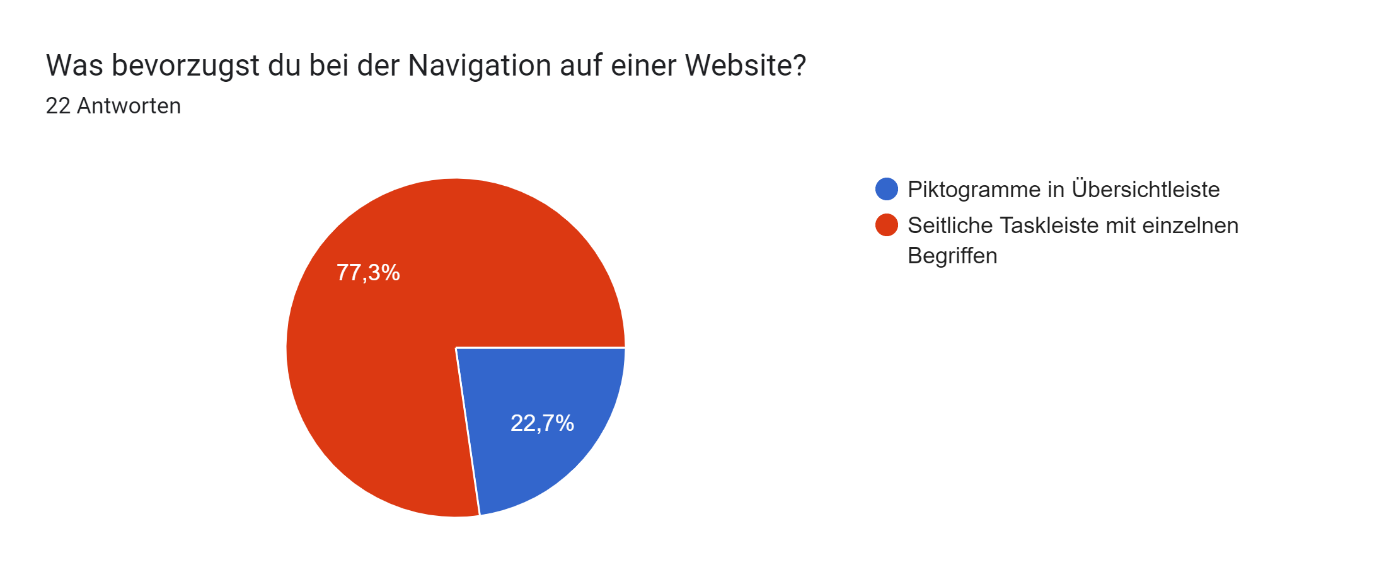
\includegraphics[width=1\textwidth]{figures/daniel/Bild-8.png}
    \caption[shortcaption]{Navigation Umfrageergebnis}
    \label{fig:bild8}
\end{figure}

\begin{figure}[!htb]
    \centering
    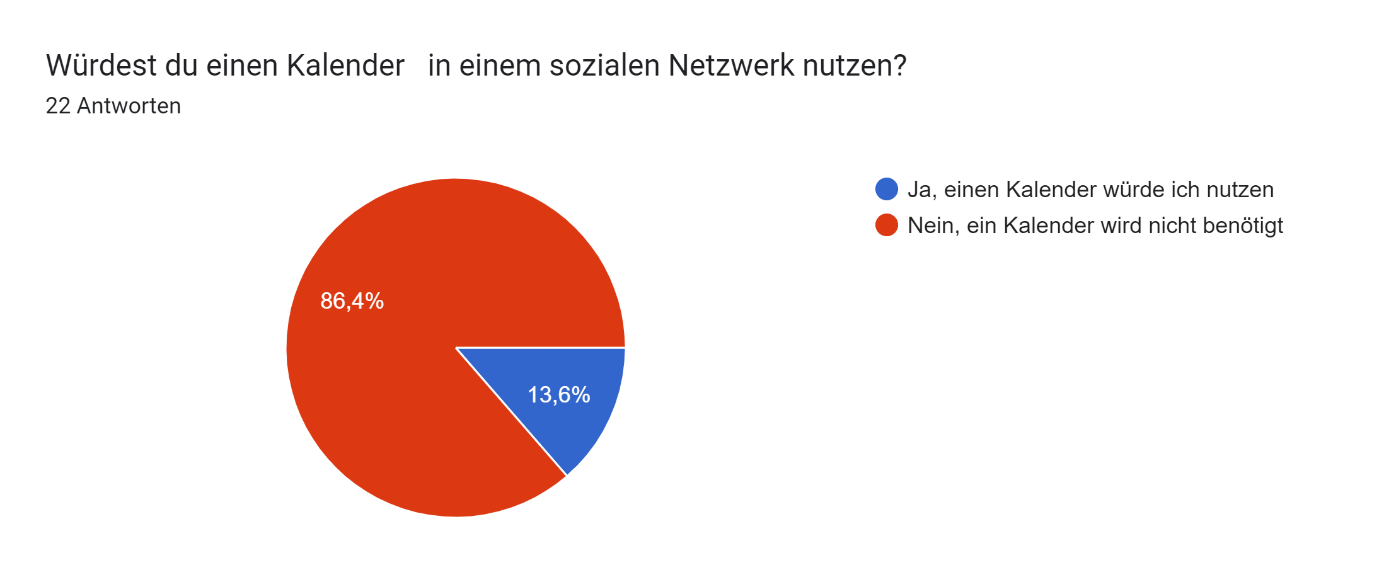
\includegraphics[width=1\textwidth]{figures/daniel/Bild-9.png}
    \caption[shortcaption]{Kalender Umfrageergebnis}
    \label{fig:bild9}
\end{figure}

\begin{figure}[!htb]
    \centering
    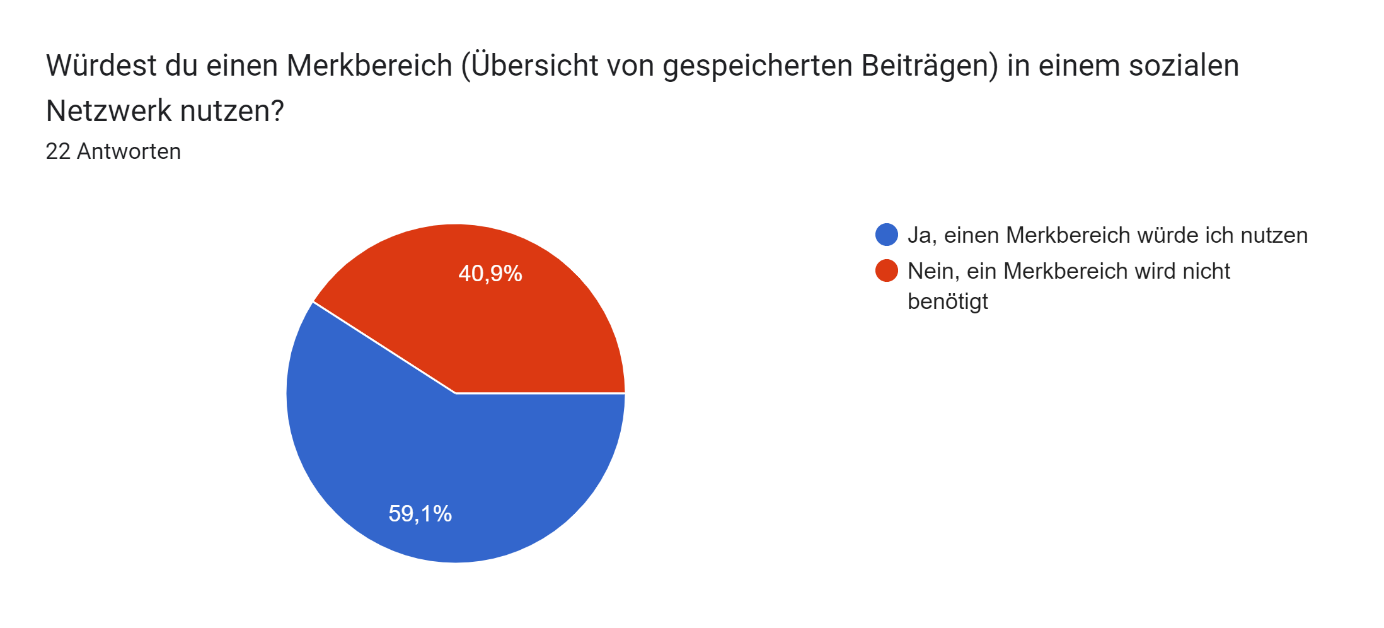
\includegraphics[width=1\textwidth]{figures/daniel/Bild-10.png}
    \caption[shortcaption]{Merkbereich Umfrageergebnis}
    \label{fig:bild10}
\end{figure}

\begin{figure}[!htb]
    \centering
    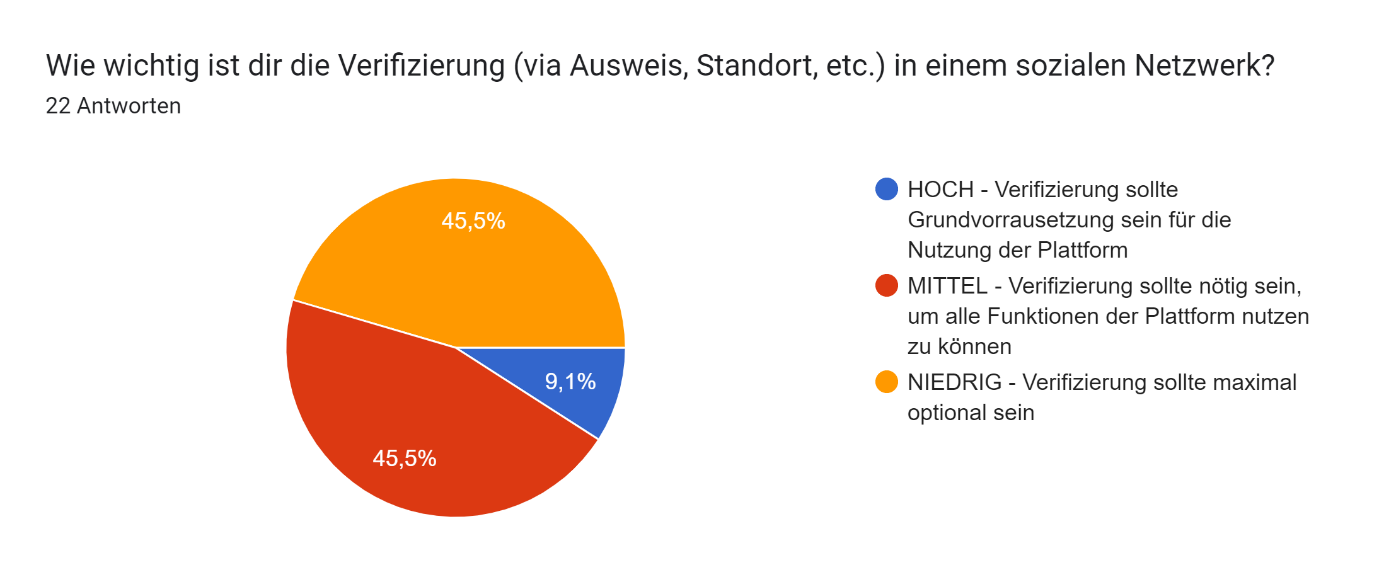
\includegraphics[width=1\textwidth]{figures/daniel/Bild-11.png}
    \caption[shortcaption]{Benutzerverifizierung Umfrageergebnis}
    \label{fig:bild11}
\end{figure}

\begin{figure}[!htb]
    \centering
    \includegraphics[width=1\textwidth]{figures/daniel/bild-12.png}
    \caption[shortcaption]{Wichtigkeit Wohnort Umfrageergebnis}
    \label{fig:bild12}
\end{figure}

\begin{figure}[!htb]
    \centering
    \includegraphics[width=1\textwidth]{figures/daniel/bild-13.png}
    \caption[shortcaption]{Kontaktiermöglichkeit Umfrageergebnis}
    \label{fig:bild13}
\end{figure}

\begin{figure}[!htb]
    \centering
    \includegraphics[width=1\textwidth]{figures/daniel/bild-14.png}
    \caption[shortcaption]{Beitragserstellung Umfrageergebnis}
    \label{fig:bild14}
\end{figure}

\begin{figure}[!htb]
    \centering
    \includegraphics[width=1\textwidth]{figures/daniel/bild-15.png}
    \caption[shortcaption]{Funktionen Beiträge Umfrageergebnis}
    \label{fig:bild15}
\end{figure}

\begin{figure}[!htb]
    \centering
    \includegraphics[width=1\textwidth]{figures/daniel/bild-16.png}
    \caption[shortcaption]{Chat Umfrageergebnis}
    \label{fig:bild16}
\end{figure}